\documentclass[11pt]{article}
\usepackage[T1]{fontenc}
\usepackage{lmodern,microtype}
\usepackage[a4paper,margin=28mm]{geometry}
\usepackage{amsmath,amssymb,amsthm,mathtools}
\usepackage{graphicx,booktabs,array,xcolor}
\usepackage[colorlinks=true,linkcolor=blue!45!black,citecolor=blue!45!black,urlcolor=blue!45!black]{hyperref}
\hypersetup{pdftitle={Centered permutation products},pdfsubject={Sharp mixed envelopes and uniform diagonal asymptotics}}
\usepackage{enumitem}
\setlist{itemsep=3pt,topsep=5pt}
\setcounter{tocdepth}{1}
\newtheorem{theorem}{Theorem}[section]
\newtheorem{proposition}[theorem]{Proposition}
\newtheorem{lemma}[theorem]{Lemma}
\newtheorem{corollary}[theorem]{Corollary}
\theoremstyle{definition}
\newtheorem{definition}[theorem]{Definition}
\newtheorem{example}[theorem]{Example}
\theoremstyle{remark}
\newtheorem{remark}[theorem]{Remark}
\newcommand{\E}{\mathbb E}
\newcommand{\PP}{\mathbb P}
\newcommand{\1}{\mathbf 1}
\newcommand{\R}{\mathbb R}
\newcommand{\NN}{\mathbb N}
\newcommand{\shc}{\operatorname{sinhc}}
\DeclareMathOperator{\tr}{tr}
\DeclareMathOperator{\diag}{diag}
\title{Centered permutation products:\\ sharp envelopes and uniform asymptotics}
\author{}
\date{November 14, 2026}
\begin{document}
\maketitle
\begin{abstract}
We prove an attained envelope for mixed centered permutation products, allowing arbitrary multiplicities and independent colors. When no conflicting centered singleton occurs, compatible cells in one permutation attain the exact maximum for fixed support and singleton counts. Scalar consequences sharpen the probabilistic estimate used in random-lift and biregular spectral-gap arguments. For distinct diagonal cells, the leading terms of Collins and Nagatsu are relatively accurate exactly when $k^3/N\to0$, answering their published optimal-scale question. The critical limits are parity-dependent hyperbolic functions. A positive partition expansion and an elementary saddle estimate give a uniform approximation throughout $k=o(N)$, a sharp hierarchy of correction thresholds, and an exact-denominator formula for every $2\le k\le N$. On bounded square-root ranges we determine the signed first error and the sharp constant in its uniform $N^{-1/4}$ rate. We explain the spectral application and isolate two failures in an intermediate conditioning formula without asserting a new graph eigenvalue theorem.
\end{abstract}
\tableofcontents
\clearpage
\section{The question and the proof mechanism}

A permutation matrix has one nonzero entry in every row and column. Its entries are therefore strongly dependent, even though each entry has mean $1/N$. This dependence has a useful consequence. Products of suitably separated centered entries are far smaller in expectation than one would predict by taking absolute values first.

For a uniform permutation matrix $M$ of size $N$, two distinct diagonal cells satisfy
\begin{equation}\label{eq:two}
\E\bigl[(M_{11}-N^{-1})(M_{22}-N^{-1})\bigr]
=\frac{1}{N(N-1)}-\frac{1}{N^2}
=\frac{1}{N^2(N-1)}.
\end{equation}
Two cells in the same row instead have centered product expectation $-N^{-2}$. The pattern of requested cells matters. The smaller scale in \eqref{eq:two} is cancellation, not independence.

The mixed-product estimate in Bordenave's Proposition 28 \cite{Bordenave} exploits this distinction. It also appears in Bordenave and Collins \cite[Proposition 22]{BC}. Brito, Dumitriu and Harris import it as Lemma 7 in their preprint, numbered Lemma 5.6 in the published article \cite{BDH}. We give a proof built from three operations:
\begin{enumerate}
\item Keep the isolated centered singletons together.
\item Condition only on a compatible set of prescribed matches. The remaining matrix is exactly a smaller uniform permutation matrix.
\item Use its row sum to obtain a positive recurrence, and only then expand the remaining factors.
\end{enumerate}
This order prevents the triangle inequality from destroying the cancellation we want to estimate.

For the diagonal product
\[
a_k(N)=\E\prod_{i=1}^k(M_{ii}-N^{-1}),
\]
Collins and Nagatsu establish the base recurrence, the parity-dependent leading terms, and the normalized error recurrences \cite[Proposition 3.3]{CN}. These are prior results. We reproduce their recurrence from a row-sum identity and use its positivity in the reverse direction, obtaining a lower bound that proves the cubic scale is necessary. A matching upper bound proves sufficiency. A continuous comparison then describes the transition itself.

\subsection{Main results at a glance}

Write $R_k=a_k/L_k$, where
\begin{equation}\label{eq:leading}
L_{2m}=(2m-1)!!N^{-3m},\qquad
L_{2m+1}=\frac{4m}{3}(2m+1)!!N^{-3m-2},\qquad m\ge1.
\end{equation}
The notation $(2m-1)!!$ means the product of the positive odd integers up to $2m-1$. The leading term for odd $k=1$ is zero, so $R_1$ is not defined.

The main conclusions are as follows.
\begin{itemize}
\item For a mixed product involving $a\le n$ distinct cells, with $h$ isolated centered singletons and $b$ nonisolated centered singletons,
\[
|\E P|\le2^b\frac{n^{-h}\mathcal P_h(n,a-h)}{(n)_a}.
\]
Here $\mathcal P_h$ is the explicit positive polynomial in \eqref{eq:depletedpoly}. When $b=0$, this is the exact maximum for fixed $n,a,h$, attained by compatible centered and raw cells in one permutation. Scalar consequences include
\[
|\E P|\le\sqrt e\,2^b n^{-a}
\left(\frac{\sqrt{a-1}}{\sqrt n-\sqrt{a-1}}\right)^h,
\qquad 2\le a\le\sqrt n.
\]
Theorem~\ref{thm:mixed} allows arbitrary multiplicities and independent colors. Corollary~\ref{cor:mixedscalar} sharpens the singleton factor when $h<a$ and proves optimality of the universal prefactor $\sqrt e$.
\item For every $2\le k\le N$,
\[
R_k-1\ge\frac{2k^3}{27N}.
\]
If $2k\le N$, then $R_k\le\exp(3k^3/N)$. Hence $R_k\to1$ exactly when $k^3/N\to0$, and $R_k=O(1)$ exactly when $k^3/N=O(1)$.
\item If $k^3/N\to c<\infty$, the even and odd ratios tend respectively to
\[
\cosh\left(\frac23\sqrt c\right),\qquad
\shc\left(\frac23\sqrt c\right),
\]
where $\shc(z)=\sinh(z)/z$ for $z\ne0$ and $\shc(0)=1$. Theorem~\ref{thm:critical} gives a uniform finite-size error.
\item With the exact parity-dependent $H_k$ in \eqref{eq:hyperdef}, the corrected formula is
\[
R_k\sim H_k\exp\{NG(\sqrt{k/N})\},\qquad
G(t)=\sum_{j\ge4}\frac{2t^j}{j(j-2)},
\]
uniformly throughout every sublinear upper range. Its first terms give sharp relative-accuracy thresholds $N^{1/2}$, $N^{3/5}$ and $N^{2/3}$. Theorem~\ref{thm:global} gives a formula at every order by keeping the denominator exact.
\item Put $W_{N,k}=R_k/[e^{k^2/(4N)}H_k]$. For every fixed $C>0$, the exact worst-case error constant is
\[
\lim_{N\to\infty}N^{1/4}
\sup_{2\le k\le C\sqrt N}|W_{N,k}-1|
=\frac{\sqrt C}{2}+\frac{2}{15}C^{5/2}.
\]
Section~\ref{sec:rates} gives the signed parity expansion and an explicit finite bound.
\end{itemize}

The mixed estimate supplies the requested probabilistic input to the graph arguments. The moment asymptotics answer a separate quantitative question about that input. They do not by themselves improve the final spectral-gap theorem.

\section{An attained envelope for mixed products}\label{sec:mixed}

Let $(\sigma_c)_c$ be independent uniform permutations of $[n]$, with $n\ge2$, and put $M_{cij}=\1_{\{\sigma_c(i)=j\}}$. A \emph{cell} is a triple $(c,i,j)$. For a nonempty set $E$ of distinct cells, assign integers $p_e,q_e\ge0$ with $p_e+q_e\ge1$, and set
\begin{equation}\label{eq:product}
P=\prod_{e\in E}(M_e-n^{-1})^{p_e}M_e^{q_e},\qquad a=|E|\le n.
\end{equation}
A cell is \emph{consistent} if no other cell of its color in $E$ shares its row or column. A \emph{centered singleton} has $(p_e,q_e)=(1,0)$. Let $h$ and $b$ count the consistent and inconsistent centered singletons, respectively. Consistency refers to the whole requested set, before a permutation is sampled.

Write $(n)_r=n(n-1)\cdots(n-r+1)$, with $(n)_0=1$, and define
\begin{equation}\label{eq:depletedpoly}
\mathcal P_j(n,r)
=j![z^j]\exp\left(\sum_{\ell\ge1}
\frac{(\ell-1)n+r}{\ell}z^\ell\right).
\end{equation}
Only a finite coefficient is extracted. The first polynomials are
$\mathcal P_0=1$, $\mathcal P_1=r$ and $\mathcal P_2=r^2+r+n$.

\begin{theorem}[An attained mixed-product envelope]\label{thm:mixed}
For the product \eqref{eq:product},
\begin{equation}\label{eq:mixedexact}
|\E P|\le 2^b\,\frac{n^{-h}\mathcal P_h(n,a-h)}{(n)_a}.
\end{equation}
For each fixed $n,a,h$, the right side with $b=0$ is the exact maximum over all permitted patterns, colors and multiplicities having these counts and no inconsistent centered singleton. It is attained by $a$ compatible cells in one color, with $h$ centered singletons and $a-h$ raw factors.
\end{theorem}

The multiplicities have no upper bound. At $a=1$, the upper bound is zero for a centered singleton and $1/n$ for every other allowed product. The scalar consequences, including the optimal $\sqrt e$ prefactor, are stated in Corollary~\ref{cor:mixedscalar}. When $n=1$ and $a\le n$, centered factors vanish and a purely raw product equals one.

\subsection{Exact depleted moments}

Fix one color and prescribe $r$ \emph{compatible} matches, meaning that their rows and columns are distinct. Their probability is $1/(n)_r$. Deleting those rows and columns leaves a uniform permutation matrix $U$ on $N=n-r$ symbols. Retain the original centering by putting $Z_{ij}=nU_{ij}-1$, whose row sum is $r$, and define
\[
\mu_j(n,r)=\E\prod_{i=1}^j Z_{ii},\qquad 0\le j\le N,\qquad \mu_0=1.
\]
Any remaining $j$ cells with distinct rows and columns have this moment after relabeling.

\begin{lemma}[Depleted row-sum recurrence]\label{lem:depleted}
For $1\le j\le n-r$,
\begin{equation}\label{eq:depleted}
(n-r-j+1)\mu_j=(r+2j-2)\mu_{j-1}+(j-1)\mu_{j-2},
\end{equation}
where the last term is omitted for $j=1$. Every $\mu_j$ is nonnegative.
\end{lemma}
\begin{proof}
Multiply the last row sum $\sum_v Z_{jv}=r$ by the preceding $j-1$ diagonal factors and take expectations. Each of the $N-j+1$ unused columns contributes $\mu_j$. For a used column $i<j$, the conflicting indicators have product zero, so
\[
Z_{ii}Z_{ji}=-Z_{ii}-Z_{ji}-1.
\]
After multiplying by the other diagonal factors, the two single-factor terms each contribute $-\mu_{j-1}$, by row relabeling, and the last contributes $-\mu_{j-2}$. Summing proves \eqref{eq:depleted}. Its denominator is positive. Induction starts with $\mu_0=1$ and, when $r<n$, $\mu_1=r/(n-r)$. At full depletion $r=n$, only the empty moment $\mu_0$ is used.
\end{proof}

For $r=0$, this is the recurrence of Collins and Nagatsu after rescaling \cite[Proposition 3.3, equation (16)]{CN}. To retain the exact moment, expand its indicators:
\[
\mu_j(n,r)=\sum_{\ell=0}^j
\binom j\ell(-1)^{j-\ell}\frac{n^\ell}{(n-r)_\ell}.
\]
Multiplication by $(n-r)_j/j!$ gives the coefficient identity
\begin{align*}
\frac{(n-r)_j\mu_j(n,r)}{j!}
&=\sum_{\ell=0}^j\frac{n^\ell}{\ell!}
(-1)^{j-\ell}\binom{n-r-\ell}{j-\ell}\\
&=[z^j](1-z)^{n-r}\exp\left(\frac{nz}{1-z}\right).
\end{align*}
Expanding the logarithm of the last generating function proves
\begin{equation}\label{eq:poly-moment}
\mu_j(n,r)=\frac{\mathcal P_j(n,r)}{(n-r)_j},
\qquad j+r\le n.
\end{equation}
This is also the classical Laguerre identity
$\mathcal P_j(n,r)=j!L_j^{(-n+r-1)}(-n)$ \cite[equation 18.12.13]{DLMF}. The coefficient derivation makes the following argument independent of that identification. Coefficients outside the moment range are only formal polynomials.

Let $\Pi_j$ denote the set partitions of $[j]$. The exponential formula in \eqref{eq:depletedpoly} reads
\begin{equation}\label{eq:depletedpartitions}
\mathcal P_j(n,r)=
\sum_{\pi\in\Pi_j}\prod_{B\in\pi}
\bigl((|B|-1)n+r\bigr)(|B|-1)!.
\end{equation}
Indeed, partitions with $m_\ell$ blocks of size $\ell$ number
$j!/\prod_\ell(\ell!)^{m_\ell}m_\ell!$. Multiplying their block weights gives exactly the coefficient in \eqref{eq:depletedpoly}.

\subsection{Merging colors and handling repeated cells}

Put
\[
F_n(r)=\frac{n^r}{(n)_r},\qquad
K_{j,r}=F_n(r)\mu_j(n,r)
=\frac{n^r\mathcal P_j(n,r)}{(n)_{j+r}}.
\]
\begin{lemma}[Monotonicity and merging]\label{lem:mixedmerge}
For fixed $n,j$, both $\mu_j(n,r)$ and $K_{j,r}$ are nondecreasing in $r$ on $0\le r\le n-j$. If $j_1+r_1+j_2+r_2\le n$, then
\[
K_{j_1,r_1}K_{j_2,r_2}\le K_{j_1+j_2,r_1+r_2}.
\]
\end{lemma}
\begin{proof}
Each block weight in \eqref{eq:depletedpartitions} increases with $r$, while $(n-r)_j$ decreases. Also the successive ratio of $n^r/(n)_{j+r}$ is $n/(n-j-r)\ge1$ whenever the next index is permitted.

For merging, unite partitions of two disjoint labeled sets and increase every block's parameter to $r_1+r_2$. Positivity gives
$\mathcal P_{j_1}(n,r_1)\mathcal P_{j_2}(n,r_2)
\le\mathcal P_{j_1+j_2}(n,r_1+r_2)$.
Finally, $(n)_u(n)_v\ge(n)_{u+v}$ when $u+v\le n$. These two comparisons prove the kernel inequality.
\end{proof}

\begin{proof}[Proof of Theorem~\ref{thm:mixed}]
Let $T$ be the $h$ consistent centered singletons. For each $e\notin T$, use $M_e^2=M_e$ to write its factor as $c_e+d_eM_e$. If $q_e\ge1$, then $c_e=0$ and $d_e=(1-1/n)^{p_e}\le1$. If $q_e=0$, then
\[
c_e=(-1/n)^{p_e},\qquad
d_e=(1-1/n)^{p_e}-(-1/n)^{p_e}\ge0.
\]
The coefficient weights satisfy
\begin{equation}\label{eq:weights}
d_e+n|c_e|\le
\begin{cases}
2,&(p_e,q_e)=(1,0),\\
1,&\text{otherwise}.
\end{cases}
\end{equation}
For the repeated centered case, put $x=1/n\le1/2$. At even $p\ge2$, the weight is at most
$(1-x)^2+(n-1)x^2=1-x$. At odd $p\ge3$, it is at most
$(1-x)^3+(n+1)x^3=1-3x+4x^2\le1-x$.
Thus repeated multiplicities cost no additional factor.

Expand the affine factors by choosing a set $S\subseteq E\setminus T$ of indicators. Incompatible choices vanish. For a compatible choice, let $r_c$ count its cells and $h_c$ the cells of $T$ in color $c$. Consistency keeps every cell of $T$ on the unexposed block. Exact conditioning gives
\begin{equation}\label{eq:prescribed}
\E\left[\prod_{e\in S}M_e
\prod_{e\in T}(M_e-n^{-1})\right]
=n^{-h-|S|}\prod_cK_{h_c,r_c}\ge0.
\end{equation}
The total index in each merge is at most $h+|S|\le a\le n$. Lemma~\ref{lem:mixedmerge} therefore gives
\[
\prod_cK_{h_c,r_c}\le K_{h,|S|}\le K_{h,a-h}.
\]
Taking absolute values of the affine coefficients and summing all subsets yields
\[
|\E P|\le n^{-a}K_{h,a-h}
\prod_{e\notin T}(d_e+n|c_e|)
\le 2^b n^{-a}K_{h,a-h}.
\]
Equation \eqref{eq:poly-moment} identifies this with \eqref{eq:mixedexact}.

For attainment, use the cells $(i,i)$, $1\le i\le a$, in one color. Center the first $h$ factors and take the other $r=a-h$ factors raw. Conditioning on the raw matches gives exactly
\[
\E P=\frac{n^{-h}\mu_h(n,r)}{(n)_r}
=\frac{n^{-h}\mathcal P_h(n,r)}{(n)_a}.
\]
This includes $h=0$, with only the empty moment at full depletion, and $a=h=1$, when the expectation is zero.
\end{proof}

\subsection{Scalar consequences and the optimal prefactor}

For $1\le h\le a\le n$, define
\begin{equation}\label{eq:mixedgamma-def}
\Gamma_{n,a,h}=
\frac{a+h-2+\sqrt{(a+h-2)^2+4(h-1)(n-a+1)}}
{2(n-a+1)}.
\end{equation}
\begin{lemma}[A geometric supersolution]\label{lem:super}
If $r+h\le a\le n$ and $h\ge1$, then
$0\le\mu_h(n,r)\le\Gamma_{n,a,h}^{\,h}$.
For $a\ge2$, put
\[
\beta=\frac{\sqrt{a-1}}{\sqrt n-\sqrt{a-1}}.
\]
Then $\Gamma_{n,a,h}\le\beta$, strictly if $h<a$, and equality holds if $h=a$. At $h=1$, $\Gamma_{n,a,1}=(a-1)/(n-a+1)$ is the exact moment at depletion $a-1$. For $h=0$, use $\mu_0=1$.
\end{lemma}
\begin{proof}
By monotonicity it suffices to use $r=a-h$. Put
$d=n-a+1$, $A=a+h-2$ and $v=h-1$. The number $\Gamma=\Gamma_{n,a,h}$ satisfies
$d\Gamma^2=A\Gamma+v$. If $\Gamma=0$, then $a=h=1$ and $\mu_1(n,0)=0$. Otherwise,
$\Gamma\ge A/d\ge r/(n-r)$.
For $2\le j\le h$, the recurrence denominator is at least $d$, and its two numerator coefficients are at most $A,v$. Induction therefore gives
\[
\mu_j\le\frac{A\Gamma^{j-1}+v\Gamma^{j-2}}d=\Gamma^j.
\]
The comparison with $\beta$ follows from
\begin{equation}\label{eq:beta}
(n-a+1)\beta^2=2(a-1)\beta+(a-1).
\end{equation}
Both right-hand coefficients increase strictly when $h<a$ is replaced by $h=a$, and the positive root increases with either coefficient. At $h=1$, the defining formula directly gives the stated first moment.
\end{proof}

\begin{corollary}[Scalar mixed bounds]\label{cor:mixedscalar}
For $h\ge1$,
\begin{equation}\label{eq:mixedgamma}
|\E P|\le 2^b n^{-a}F_n(a-h)\Gamma_{n,a,h}^{\,h}.
\end{equation}
For $2\le a\le n$ and every $h$,
\begin{equation}\label{eq:mixedgeneral}
|\E P|\le F_n(a-h)\,2^b n^{-a}\beta^h
\le\exp\left(\frac{a(a-1)}{2(n-a+1)}\right)2^bn^{-a}\beta^h.
\end{equation}
If $2\le a\le\sqrt n$, then
\begin{equation}\label{eq:mixedmain}
|\E P|\le\sqrt e\,2^b n^{-a}\beta^h
\le\sqrt e\,2^b n^{-a}\left(2\sqrt{a/n}\right)^h.
\end{equation}
The universal prefactor $\sqrt e$ in \eqref{eq:mixedmain} is optimal for this class.
\end{corollary}
\begin{proof}
The exact bound is $2^bn^{-a}F_n(a-h)\mu_h(n,a-h)$. Apply Lemma~\ref{lem:super}, with $\mu_0=1$ when $h=0$.

The elementary raw factorial estimate giving $\sqrt e$ is already recorded by Bordenave and Zhu \cite[Lemma 2.1, equation (2.3)]{BZ}. Here, for $0\le q\le a$, the inequality $-\log(1-x)\le x/(1-x)$ gives
\[
\log F_n(q)\le\frac{q(q-1)}{2(n-q+1)}
\le\frac{a(a-1)}{2(n-a+1)}.
\]
This is one global factor after the color merge. If $a^2\le n$, the last expression is at most $1/2$. Also $\sqrt{(a-1)/n}\le1/2$, so $\beta\le2\sqrt{a/n}$.

For sharpness, take $n=a^2$ and $a$ compatible raw cells in one color. Then $h=b=0$ and $n^a\E P=F_{a^2}(a)$, while
\[
\log F_{a^2}(a)=
\sum_{j=0}^{a-1}-\log(1-j/a^2)
=\frac{a(a-1)}{2a^2}+O(a^{-1})\longrightarrow\frac12.
\]
Thus no smaller universal prefactor works in \eqref{eq:mixedmain}.
\end{proof}

\subsection{Dependence on the product's composition}

For each fixed $h\ge1$, if $n\to\infty$ and $r/\sqrt n\to\rho\ge0$, then
\begin{equation}\label{eq:mixedfixedh}
n^{h/2}\mu_h(n,r)\longrightarrow
g_h(\rho)=h!\sum_{q=0}^{\lfloor h/2\rfloor}
\frac{\rho^{h-2q}}{(h-2q)!\,2^q q!}.
\end{equation}
Indeed, in the finite partition sum \eqref{eq:depletedpartitions}, singleton and pair weights are $r$ and $n+r$. After division by $n^{h/2}$ they have the displayed limits. Every block of size $\ell\ge3$ contributes a vanishing factor $O(n^{1-\ell/2})$. Finally, $(n-r)_h/n^h\to1$.

For example, take $n=a^2$, $r=a-h$ and fixed $h$ as $a\to\infty$. Then
\[
\frac{\mu_h(a^2,a-h)}{\beta^h}
\sim g_h(1)a^{-h/2},
\qquad
\Gamma_{a^2,a,h}\sim\frac{1+\sqrt{4h-3}}{2a}.
\]
This compares the full bounds, whose other factors coincide. The attaining family in Theorem~\ref{thm:mixed} realizes the improved order.

Such an improvement is not uniform when all singleton counts grow. For even $h=a$, pair partitions give
\[
\mu_a(n,0)\ge(a-1)!!\,n^{-a/2}
\ge\left(\frac{a}{en}\right)^{a/2}.
\]
The second inequality follows by summing the midpoint bound for $\log(2x)$ over $[0,a/2]$. Hence, along even $a\to\infty$ with $a^2\le n$, no fixed universal prefactor permits a singleton scale $o(\sqrt{a/n})$.

Finally, colors may have separate dimensions. If color $c$ has dimension $n_c\ge2$, centering $1/n_c$, and local counts $a_c,h_c,b_c$ with $a_c\le n_c$, independence gives
\begin{equation}\label{eq:mixed-dimensions}
|\E P|\le\prod_c
\left[
2^{b_c}\frac{n_c^{-h_c}\mathcal P_{h_c}(n_c,a_c-h_c)}
{(n_c)_{a_c}}
\right].
\end{equation}
There is no restriction on $\sum_c a_c$. If every $b_c=0$, compatible centered and raw choices attain all local bounds simultaneously, so \eqref{eq:mixed-dimensions} is again an exact maximum for the specified local counts.

\section{The exact cubic threshold}\label{sec:threshold}

We now study $a_k(N)$ and $R_k=a_k/L_k$ from \eqref{eq:leading}, always with $2\le k\le N$. The matrix size is denoted by $N$ to distinguish this analysis from the depleted permutation in Section~\ref{sec:mixed}.

\begin{theorem}[Necessary and sufficient scale]\label{thm:threshold}
For every $2\le k\le N$,
\begin{equation}\label{eq:lower}
R_k-1\ge\frac{2k^3}{27N}.
\end{equation}
For $2k\le N$,
\begin{equation}\label{eq:upper}
R_k\le\exp(3k^3/N).
\end{equation}
Consequently, for every integer sequence $2\le k_N\le N$ as $N\to\infty$,
\begin{align}
R_{k_N}\to1&\quad\Longleftrightarrow\quad k_N^3/N\to0,\label{eq:iff}\\
R_{k_N}=O(1)&\quad\Longleftrightarrow\quad k_N^3/N=O(1).\label{eq:bounded}
\end{align}
The lower-bound constant $2/27$ is optimal uniformly over both parities.
\end{theorem}

The necessity in this result addresses the question in Collins and Nagatsu's published Remark 3.4 \cite{CN}. The statement concerns relative accuracy of their specific leading terms. It does not say that centered products cease to have useful upper bounds outside the cubic range.

\subsection{The known recurrence and its normalization}

Lemma~\ref{lem:depleted} with $r=0$, after rescaling, gives
\begin{equation}\label{eq:momentrec}
a_k=\frac{2(k-1)}{N(N-k+1)}a_{k-1}
+\frac{k-1}{N^2(N-k+1)}a_{k-2},
\qquad a_0=1,\quad a_1=0.
\end{equation}
This is \cite[equation (16)]{CN}. Its coefficients show that $a_k>0$ for $2\le k\le N$.

Set $E_k=R_k-1$. Substitution of \eqref{eq:leading} into \eqref{eq:momentrec} gives the following normalized recurrences, also present in the proof of \cite[Proposition 3.3]{CN}. For $m\ge2$,
\begin{align}
E_{2m}={}&\frac{N}{N-2m+1}E_{2m-2}
+\frac{4(2m-1)(2m-2)}{3(N-2m+1)}E_{2m-1}\notag\\
&+\frac{(2m-1)(8m-5)}{3(N-2m+1)}.\label{eq:evenerror}
\end{align}
For $m\ge1$,
\begin{align}
E_{2m+1}={}&\frac{3N}{(N-2m)(2m+1)}E_{2m}
+\frac{(2m-2)N}{(N-2m)(2m+1)}E_{2m-1}
+\frac{2m}{N-2m},\label{eq:odderror}
\end{align}
where the term involving $E_1$ is omitted at $m=1$. The initial error is $E_2=1/(N-1)$. Every coefficient and forcing term is nonnegative. In particular, $E_k\ge0$.

\subsection{Accumulating a lower bound}

In \eqref{eq:evenerror}, discard the second nonnegative term and bound the other denominator by $N$. This gives
\[
E_{2m}\ge E_{2m-2}+\frac{(2m-1)(8m-5)}{3N}.
\]
At $m=1$, the same inequality means $E_2\ge1/N$, with $E_0=0$ used only for the summation. Summing yields
\begin{equation}\label{eq:evenlower}
E_{2m}\ge\frac{C_{\rm e}(m)}N,
\qquad C_{\rm e}(m)=\frac{m(16m^2-3m-4)}9.
\end{equation}
The right side is at least $m^3/N$, because
\[
C_{\rm e}(m)-m^3=\frac{m(m-1)(7m+4)}9\ge0.
\]

For the odd orders define
\[
C_{\rm o}(m)=\frac{80m^3+195m^2+124m+6}{135}.
\]
A direct polynomial calculation gives $C_{\rm o}(1)=3$ and
\begin{equation}\label{eq:oddpoly}
C_{\rm o}(m)=\frac{3C_{\rm e}(m)+(2m-2)C_{\rm o}(m-1)}{2m+1}+2m.
\end{equation}
Equation~\eqref{eq:odderror} implies
\[
E_{2m+1}\ge\frac{3E_{2m}+(2m-2)E_{2m-1}}{2m+1}+\frac{2m}N.
\]
Induction using \eqref{eq:evenlower} and \eqref{eq:oddpoly} proves
\begin{equation}\label{eq:oddlower}
E_{2m+1}\ge C_{\rm o}(m)/N.
\end{equation}
At $m=1$, this starts from $E_3\ge E_2+2/N\ge3/N$. Finally,
\[
C_{\rm o}(m)-\frac{2(2m+1)^3}{27}
=\frac{75m^2+64m-4}{135}>0.
\]
For the even orders, $m^3\ge2(2m)^3/27$. Together these inequalities prove \eqref{eq:lower}.

\subsection{A self-contained upper bound}

Suppose $2k\le N$. In the recurrences for $R_j$, obtained by adding one back to \eqref{eq:evenerror} and \eqref{eq:odderror}, the sum of the coefficients is
\[
1+\frac{(2m-1)(8m-5)}{3(N-2m+1)}
\quad\text{for }j=2m,
\]
and $N/(N-2m)$ for $j=2m+1$. In both cases it is at most $1+3j^2/N$, using $N-j+1\ge N/2$. The same bound starts the induction at $R_2=N/(N-1)$. Positivity gives
\[
\max(1,R_2,\ldots,R_k)
\le\prod_{j=2}^k(1+3j^2/N)
\le\exp\left(\frac3N\sum_{j=2}^k j^2\right)
\le\exp(3k^3/N).
\]
This proves \eqref{eq:upper}.

If $k_N^3/N\to0$ or merely stays bounded, then $2k_N\le N$ eventually. The two bounds now imply \eqref{eq:iff} and \eqref{eq:bounded}. Sharpness of $2/27$ follows from Corollary~\ref{cor:small} below.

\begin{example}[Order four]
The recurrence gives
\[
a_4(N)=\frac{3(N+6)}{N^4(N-1)(N-2)(N-3)},\qquad
R_4(N)=\frac{N^2(N+6)}{(N-1)(N-2)(N-3)}.
\]
Thus $R_4=1+12/N+O(N^{-2})$. A fixed-order expansion like this is useful for checking normalization. The threshold theorem needs the uniform argument above, because its order is allowed to grow with $N$.
\end{example}

\section{The critical transition and its parity}\label{sec:critical}

The cubic threshold is visible in the normalized recurrence: the even ratio changes by order $m^2/N$ at step $m$, and summing this over $m$ steps produces $m^3/N$. At the transition, these increments cannot be discarded. They converge to a coupled differential system.

\begin{theorem}[Uniform critical approximation]\label{thm:critical}
For every fixed $T>0$ there is a finite $C_T$ such that, whenever $M\ge1$, $N\ge4M+2$ and $M^3/N\le T$,
\begin{align}
\max_{1\le m\le M}\left|R_{2m}-\cosh z_m\right|&\le C_T M^2/N,\label{eq:criticeven}\\
\max_{1\le m\le M}\left|R_{2m+1}-\shc z_m\right|&\le C_T M^2/N,\label{eq:criticodd}
\end{align}
where $z_m=(4\sqrt2/3)\sqrt{m^3/N}$. If $k_N^3/N\to c\in[0,\infty)$, then
\begin{align*}
R_{k_N}&\longrightarrow\cosh\left(\frac23\sqrt c\right)
&&\text{along even orders},\\
R_{k_N}&\longrightarrow\shc\left(\frac23\sqrt c\right)
&&\text{along odd orders at least three}.
\end{align*}
For $c>0$, the two limits are different.
\end{theorem}

\subsection{The exact two-component recursion}

Put $e_m=R_{2m}$ and $o_m=R_{2m+1}$ for $m\ge1$, with auxiliary seeds $e_0=o_0=1$. These seeds do not define $R_0$ or $R_1$. The coefficients multiplying $o_0$ vanish at the first step. Equation~\eqref{eq:momentrec} gives
\begin{equation}\label{eq:tworec}
e_m=A_me_{m-1}+B_mo_{m-1},\qquad
o_m=C_me_m+D_mo_{m-1},
\end{equation}
where
\begin{align*}
A_m&=\frac N{N-2m+1},&
B_m&=\frac{4(2m-1)(2m-2)}{3(N-2m+1)},\\
C_m&=\frac{3N}{(N-2m)(2m+1)},&
D_m&=\frac{(2m-2)N}{(N-2m)(2m+1)}.
\end{align*}
At $m=1$, these reproduce $R_2=N/(N-1)$ and $R_3=N^2/((N-1)(N-2))$. Under $N\ge4M+2$, all coefficients are nonnegative and
\begin{equation}\label{eq:rowsums}
A_m+B_m\le1+12m^2/N,\qquad
C_m+D_m\le1+4m^2/N,\qquad C_m\le2.
\end{equation}
For example, the first row sum has excess
\[
\frac{(2m-1)(8m-5)}{3(N-2m+1)}\le\frac{32m^2}{3N}.
\]
The second row sum is $N/(N-2m)$, with excess at most $4m/N$.

\subsection{A comparison system with an explicit solution}

For $x\ge0$ set
\[
z(x)=\frac{4\sqrt2}{3}\sqrt{x^3/N},\qquad
E(x)=\cosh z(x),\qquad O(x)=\shc z(x).
\]
Direct differentiation gives
\begin{equation}\label{eq:ode}
E'(x)=\frac{16x^2}{3N}O(x),\qquad
O'(x)=\frac3{2x}(E(x)-O(x)).
\end{equation}
The second identity extends continuously to $x=0$. The associated power series are
\[
E(x)=\sum_{\ell\ge0}\frac{(32x^3/(9N))^\ell}{(2\ell)!},\qquad
O(x)=\sum_{\ell\ge0}\frac{(32x^3/(9N))^\ell}{(2\ell+1)!}.
\]
For $x^3/N\le T$, termwise differentiation therefore gives
\begin{align}
|E(x)|+|O(x)|&\le K_T,&
|E(x)-O(x)|&\le K_Tx^3/N,\notag\\
|E'(x)|+|O'(x)|&\le K_Tx^2/N,&
|E''(x)|+|O''(x)|&\le K_Tx/N.\label{eq:derivatives}
\end{align}
The derivative estimates follow by factoring $x^2/N$ or $x/N$ from the differentiated series. The remaining series converge uniformly on the bounded interval for $x^3/N$.

\subsection{Local errors and stability}

Write $E_m=E(m)$ and $O_m=O(m)$. The residuals of \eqref{eq:tworec} are
\[
\rho_m^E=E_m-A_mE_{m-1}-B_mO_{m-1},\qquad
\rho_m^O=O_m-C_mE_m-D_mO_{m-1}.
\]
We claim that
\begin{equation}\label{eq:residual}
|\rho_m^E|+|\rho_m^O|\le K'_Tm/N.
\end{equation}
Taylor's theorem and \eqref{eq:derivatives} bound each backward difference minus its derivative at $m$ by $O_T(m/N)$. With $b_m=16m^2/(3N)$, the exact coefficients give
\[
A_m-1=O(m/N),\qquad B_m-b_m=O_T(m/N).
\]
For the second estimate, direct subtraction bounds the difference by a constant times $m/N+m^3/N^2$, which is $O_T(m/N)$. Now
\begin{align*}
\rho_m^E={}&E_m-E_{m-1}-E'(m)+b_m(O_m-O_{m-1})\\
&-(A_m-1)E_{m-1}-(B_m-b_m)O_{m-1}.
\end{align*}
Every term is $O_T(m/N)$. In particular, the second term is $O_T(m^4/N^2)$, and $m^3/N\le T$ makes it $O_T(m/N)$.

For the odd residual write
\[
c_m=\frac3{2m+1},\quad d_m=\frac{2m-2}{2m+1},\quad t_m=\frac N{N-2m}.
\]
Then $c_m+d_m=1$, $C_m=t_mc_m$, $D_m=t_md_m$ and $t_m-1=O(m/N)$. Removing $t_m$ changes the residual by $O_T(m/N)$. The remaining expression is
\[
d_m(O_m-O_{m-1})-c_m(E_m-O_m).
\]
After substituting \eqref{eq:ode}, the coefficient of $E_m-O_m$ is
\[
d_m\frac3{2m}-c_m=-\frac3{m(2m+1)}.
\]
Equation~\eqref{eq:derivatives} bounds its contribution by $O_T(m/N)$, proving \eqref{eq:residual}, including at $m=1$.

Let $H_m=\max(|e_m-E_m|,|o_m-O_m|)$ and $H_0=0$. Subtract the comparison equations from \eqref{eq:tworec}. First bound the even error, then use that bound in the odd equation. Positivity and \eqref{eq:rowsums} yield
\[
H_m\le(1+12m^2/N)(1+4m^2/N)H_{m-1}+3K'_Tm/N.
\]
The product of all multiplicative factors through step $M$ is at most
\[
\exp\left(\frac{16}N\sum_{m=1}^M m^2\right)\le e^{16T}.
\]
Summing the local errors proves $\max_{m\le M}H_m\le3K'_Te^{16T}M^2/N$, establishing \eqref{eq:criticeven} and \eqref{eq:criticodd}.

If $k^3/N$ stays bounded, then $m=O(N^{1/3})$ and the error tends to zero. For even $k=2m$, $z_m^2=4k^3/(9N)$. For odd $k=2m+1$, replacing $(2m)^3/N$ by $k^3/N$ changes it by $O(m^2/N)$. Continuity proves the stated limits.

\begin{corollary}[Small relative errors and sharpness]\label{cor:small}
If $k\to\infty$ and $k^3/N\to0$, then
\[
R_k-1\sim\frac{2k^3}{9N}\quad\text{for even }k,
\qquad
R_k-1\sim\frac{2k^3}{27N}\quad\text{for odd }k.
\]
Thus the constant $2/27$ in Theorem~\ref{thm:threshold} cannot be increased.
\end{corollary}
\begin{proof}
Take a fixed $T$, for instance $T=1$. The error $O(M^2/N)$ with $M$ equal to the relevant $m$ is smaller than $k^3/N$ by a factor of order $1/k$. Expand $\cosh z=1+z^2/2+O(z^4)$ and $\shc z=1+z^2/6+O(z^4)$.
\end{proof}

\begin{example}[A transition visible without a large formula]
When $k^3/N\to9/4$, the two limits are $\cosh(1)\approx1.5431$ and $\sinh(1)\approx1.1752$. Both exceed one. Their difference shows why an arbitrary sequence containing both parities need not have a common normalized limit.
\end{example}

\section{Positive partitions and a wider asymptotic window}\label{sec:extension}

The recurrence admits a positive coefficient representation. It explains the hyperbolic functions by counting pairs and triples, and extends their relative accuracy well beyond the critical cubic range. At the square-root scale, a further correction becomes visible.

For $k\ge2$, put $m=\lfloor k/2\rfloor$, $K=2m$ and
\begin{equation}\label{eq:hyperdef}
\lambda=\frac23\sqrt{K^3/N},\qquad
H_k=\begin{cases}\cosh\lambda,&k\text{ even},\\
\shc\lambda,&k\text{ odd}.
\end{cases}
\end{equation}
For odd $k$, the definition intentionally uses $K=k-1$.



\begin{theorem}[Relative hyperbolic approximation]\label{thm:window}
For integers $2\le k\le N/4$,
\begin{equation}\label{eq:envelope}
\left(1-\frac{4k^2}{3N}\right)H_k
\le R_k\le e^{4k^2/N}H_k.
\end{equation}
If $4k^2\le N$, then
\begin{equation}\label{eq:logerror}
-\frac{2k^2}N\le\log\frac{R_k}{H_k}\le\frac{4k^2}N.
\end{equation}
Consequently $R_k/H_k\to1$ whenever $k=o(\sqrt N)$, even if $k^3/N\to\infty$.
\end{theorem}

\begin{theorem}[The square-root correction]\label{thm:sqrt}
If $k^2/N\to d\in(0,\infty)$, then
\begin{equation}\label{eq:sqrtlimit}
\frac{R_k}{H_k}\longrightarrow e^{d/4}.
\end{equation}
For every fixed $C>0$,
\begin{equation}\label{eq:uniformsqrt}
\sup_{2\le k\le C\sqrt N}
\left|\frac{R_k}{e^{k^2/(4N)}H_k}-1\right|\longrightarrow0,
\end{equation}
where the supremum is over integers and $N\to\infty$.
\end{theorem}

Thus the uncorrected hyperbolic approximation loses relative accuracy at every positive square-root scale. The corrected expression is uniformly accurate on bounded multiples of that scale. Sections~\ref{sec:asymptotics} and~\ref{sec:rates} extend its range and determine its sharp first error.

\subsection{Clearing the denominators}

Set $Q_k=(N)_kN^ka_k$, with $Q_0=1$ and $Q_1=0$. Equation~\eqref{eq:momentrec} becomes
\begin{equation}\label{eq:qrec}
Q_k=2(k-1)Q_{k-1}+(k-1)(N-k+2)Q_{k-2}.
\end{equation}
Extend this polynomial recurrence formally to all orders. This algebraic extension does not define permutation moments for $k>N$. The exponential generating function $F(z)=\sum_{k\ge0}Q_kz^k/k!$ satisfies
\[
(1-z)^2F'(z)=NzF(z),\qquad F(0)=1.
\]
Consequently,
\begin{equation}\label{eq:egf}
F(z)=\exp\left(N\left[\frac z{1-z}+\log(1-z)\right]\right)
=\exp\left(N\sum_{j\ge2}\frac{j-1}{j}z^j\right).
\end{equation}
This is a classical Laguerre generating function: $Q_k=k!L_k^{(-N-1)}(-N)$ \cite[equations 18.5.12 and 18.12.13]{DLMF}. It is also a reformulation of the special-function identification in \cite[Remark 3.5]{CN}. We derive it here to use its positive coefficients, not as a new special-function identity.

Extracting coefficients gives
\begin{equation}\label{eq:partitions}
Q_k=k!\sum_{\substack{c_2,c_3,\ldots\ge0\\\sum_{j\ge2}jc_j=k}}
\prod_{j\ge2}\frac{(N(j-1)/j)^{c_j}}{c_j!}.
\end{equation}
Equivalently, this is a weighted count of labeled set partitions without singleton blocks. A block of size $j$ has weight $N(j-1)(j-1)!$. Pairs have weight $N$, and triples have weight $4N$.

Define the polynomial leading terms
\[
\mathcal L_{2m}=(2m-1)!!N^m,\qquad
\mathcal L_{2m+1}=\frac{4m}{3}(2m+1)!!N^m.
\]
They count all-pair partitions and one-triple partitions, respectively. Indeed, the latter coefficient is
\[
\binom{2m+1}{3}4(2m-3)!!=\frac{4m}{3}(2m+1)!!.
\]
With $D_k=N^k/(N)_k$, the normalization is exactly
\begin{equation}\label{eq:qnormalize}
R_k=D_k\frac{Q_k}{\mathcal L_k}.
\end{equation}

\subsection{The number of available pairs}

For blocks of size at least three put
\[
S=\sum_{j\ge3}jc_j,\qquad x=\sqrt{K/N},\qquad
\lambda_j=N\frac{j-1}{j}x^j.
\]
In particular, $\lambda_3=\lambda$. Cancelling the pair factorial in \eqref{eq:partitions} against the one in $\mathcal L_k$, the normalized contribution of these nonpair counts is
\begin{equation}\label{eq:availabilityeven}
\frac{(m)_{S/2}}{m^{S/2}}
\prod_{j\ge3}\frac{\lambda_j^{c_j}}{c_j!}
\quad\text{if }k=2m\text{ and }S\text{ is even},
\end{equation}
and
\begin{equation}\label{eq:availabilityodd}
\frac{(m-1)_{(S-3)/2}}{m^{(S-3)/2}}
\frac1\lambda\prod_{j\ge3}\frac{\lambda_j^{c_j}}{c_j!}
\quad\text{if }k=2m+1\text{ and }S\text{ is odd}.
\end{equation}
An odd $S$ here is at least three. A falling factorial with too many factors is assigned zero. The availability factors lie in $[0,1]$ and enforce the requirement that enough pairs remain.

\subsection{Proof of the finite relative bounds}

Assume $k\le N/4$, so $x\le1/2$. Put
\[
A_* =\sum_{\substack{j\ge4\\j\text{ even}}}\lambda_j,
\qquad B_* =\sum_{\substack{j\ge3\\j\text{ odd}}}\lambda_j.
\]
Remove the availability factors and project the exponential series onto the required parity. This gives
\[
\frac{Q_{2m}}{\mathcal L_{2m}}\le e^{A_*}\cosh B_*,\qquad
\frac{Q_{2m+1}}{\mathcal L_{2m+1}}\le e^{A_*}\frac{\sinh B_*}{\lambda}.
\]
The extra block weights satisfy
\begin{align*}
A_*+B_*-\lambda&\le\frac{Nx^4}{1-x}\le\frac{2K^2}N,\\
\frac{B_*}{\lambda}&\le1+\frac{3x^2}{2(1-x^2)}
\le1+\frac{2K}N\le e^{K^2/N}.
\end{align*}
The logarithmic derivatives of $\cosh t$ and $\shc t$ lie in $[0,1]$ for $t>0$. For the latter this follows from $0\le\coth t-1/t\le1$. Thus
\[
Q_k/\mathcal L_k\le e^{3K^2/N}H_k.
\]
Also
\[
\log D_k\le\frac{k(k-1)}{2(N-k+1)}\le k^2/N.
\]
Equation~\eqref{eq:qnormalize} proves the upper bound in \eqref{eq:envelope}.

For the lower bound, retain only pairs and triples. At even order, with $J$ triples,
\[
\frac{Q_{2m}}{\mathcal L_{2m}}
\ge\sum_{\ell\ge0}\frac{\lambda^{2\ell}}{(2\ell)!}
\frac{(m)_{3\ell}}{m^{3\ell}}.
\]
For any integer $s\ge0$,
\[
\frac{(m)_s}{m^s}\ge1-\frac{s(s-1)}{2m}.
\]
This follows from the product bound $\prod_i(1-u_i)\ge1-\sum_i u_i$ for $0\le u_i\le1$. If $s>m$, the left side is zero and the right side is nonpositive.

Normalize $\lambda^J/J!$ on even $J$ by $\cosh\lambda$. Then
\[
\E J=\lambda\tanh\lambda,\qquad
\E J^2=\lambda^2+\lambda\tanh\lambda.
\]
With $s=3J/2$, the relative loss is at most
\[
\frac{9\lambda^2+3\lambda\tanh\lambda}{8m}
\le\frac{3\lambda^2}{2m}=\frac{4K^2}{3N}.
\]
For odd order the analogous series is
\[
\frac{Q_{2m+1}}{\mathcal L_{2m+1}}
\ge\sum_{\ell\ge0}\frac{\lambda^{2\ell}}{(2\ell+1)!}
\frac{(m-1)_{3\ell}}{m^{3\ell}}.
\]
Now $(m-1)_s/m^s\ge1-s(s+1)/(2m)$. Normalize $\lambda^J/J!$ on odd $J$ by $\sinh\lambda$ and use $s=3(J-1)/2$. The relative loss is at most
\[
\frac{9\lambda^2-3\lambda\coth\lambda+3}{8m}
\le\frac{9\lambda^2}{8m}=\frac{K^2}N,
\]
because $\lambda\coth\lambda\ge1$. Multiplying by $D_k\ge1$ proves the lower half of \eqref{eq:envelope}. If its factor is negative, positivity suffices. Finally, $\log(1-4u/3)\ge-2u$ for $0\le u\le1/4$, proving \eqref{eq:logerror} and Theorem~\ref{thm:window}.

\subsection{Proof of the square-root correction}

Suppose $k^2/N\to d\in(0,\infty)$. Let $C_j$, $j\ge3$, be independent Poisson variables with means $\lambda_j$, and put
\[
\Lambda=\sum_{j\ge3}\lambda_j,\qquad S=\sum_{j\ge3}jC_j.
\]
For all sufficiently large $N$, $x<1$, so the total mean is finite and only finitely many $C_j$ are nonzero almost surely. Define
\[
w_{\rm e}(s)=(m)_s/m^s\quad(0\le s\le m),\qquad
w_{\rm o}(s)=(m-1)_s/m^s\quad(0\le s\le m-1),
\]
with value zero outside the respective integer ranges. The exact sums \eqref{eq:availabilityeven} and \eqref{eq:availabilityodd} become
\begin{align}
\frac{Q_{2m}}{\mathcal L_{2m}}
&=e^\Lambda\E\bigl[\1_{\{S\text{ even}\}}w_{\rm e}(S/2)\bigr],\label{eq:poissoneven}\\
\frac{Q_{2m+1}}{\mathcal L_{2m+1}}
&=\frac{e^\Lambda}{\lambda}\E\bigl[\1_{\{S\text{ odd}\}}w_{\rm o}((S-3)/2)\bigr].\label{eq:poissonodd}
\end{align}
Each availability function is evaluated only on its displayed parity event.

First control all block sizes:
\[
\lambda\to\infty,\qquad
\lambda_4=\frac{3K^2}{4N}\to\frac{3d}4,\qquad
\sum_{j\ge5}\lambda_j\le\frac{Nx^5}{1-x}\to0.
\]
Therefore $C_3/\lambda\to1$ in probability, $C_4=O_{\PP}(1)$, and the probability of any larger block tends to zero. Also $\Lambda-\lambda\to3d/4$.

On the event of no larger block, the argument $s$ of either availability function is $3C_3/2+2C_4+O(1)$. Since $\lambda^2/m\to8d/9$, we obtain, on the relevant parity event,
\[
\frac{s^2}{2m}\to d,\qquad \frac sm\to0,\qquad \frac{s^3}{m^2}\to0
\]
in probability. For $s/m\le1/2$, expansion of the logarithm gives
\[
\log w_{\rm e}(s)=-\frac{s(s-1)}{2m}+O(s^3/m^2),\qquad
\log w_{\rm o}(s)=-\frac{s(s+1)}{2m}+O(s^3/m^2).
\]
For example, these follow by summing
$0\le-\log(1-u)-u\le u^2/(2(1-u))$.
Thus each availability factor approaches $e^{-d}$ on its relevant parity event. All factors lie in $[0,1]$, so the corresponding error multiplied by the parity indicator tends to zero in mean.

The Poisson parity identity gives
\[
\PP(S\text{ even})=\frac{1+e^{-2B_*}}2,\qquad
\PP(S\text{ odd})=\frac{1-e^{-2B_*}}2.
\]
Because $B_*\ge\lambda\to\infty$, both probabilities tend to $1/2$. Hence both expectations in \eqref{eq:poissoneven} and \eqref{eq:poissonodd} tend to $e^{-d}/2$. No independence between parity and availability is required.

Since $\cosh\lambda\sim e^\lambda/2$ and $\sinh\lambda\sim e^\lambda/2$,
\[
\frac{Q_k/\mathcal L_k}{H_k}\longrightarrow e^{3d/4-d}=e^{-d/4}.
\]
Finally,
\[
\log D_k=\frac{k(k-1)}{2N}+O(k^3/N^2)\longrightarrow d/2.
\]
Restoring $D_k$ in \eqref{eq:qnormalize} proves \eqref{eq:sqrtlimit}. The three contributions are $3d/4$ from four-blocks, $-d$ from pair depletion and $d/2$ from the permutation probability.

To prove \eqref{eq:uniformsqrt}, suppose its supremum failed to tend to zero. Select a sequence of offending orders and pass to a subsequence on which $k^2/N\to d\in[0,C^2]$. If $d=0$, Theorem~\ref{thm:window} gives convergence to one. If $d>0$, \eqref{eq:sqrtlimit} gives it. Both contradict the selection.

\subsection{A worked partition count}

The first polynomials include
\[
Q_2=N,\quad Q_3=4N,\quad Q_4=3N^2+18N,\quad
Q_6=15N^3+430N^2+600N.
\]
For $Q_6$, the four contributions are
\begin{center}
\begin{tabular}{lr}
\toprule
Block sizes & Contribution\\
\midrule
$2+2+2$ & $15N^3$\\
$3+3$ & $160N^2$\\
$2+4$ & $270N^2$\\
$6$ & $600N$\\
\bottomrule
\end{tabular}
\end{center}
At the cubic scale, triples have bounded effective weight, while four-blocks and pair depletion disappear. Summing an even or odd number of triples gives the two hyperbolic functions. At the square-root scale, the four-block weight and pair depletion survive, producing the correction in Theorem~\ref{thm:sqrt}.

In the intermediate regime $N^{1/3}\ll k\ll\sqrt N$, Theorem~\ref{thm:window} also yields
\[
R_k\sim\tfrac12e^\lambda\quad(k\text{ even}),\qquad
R_k\sim\frac{e^\lambda}{2\lambda}\quad(k\text{ odd}).
\]
At $k\sim\sqrt N$, the ratio to the uncorrected hyperbolic term tends instead to $e^{1/4}\approx1.2840$.

\begin{figure}[htbp]
\centering
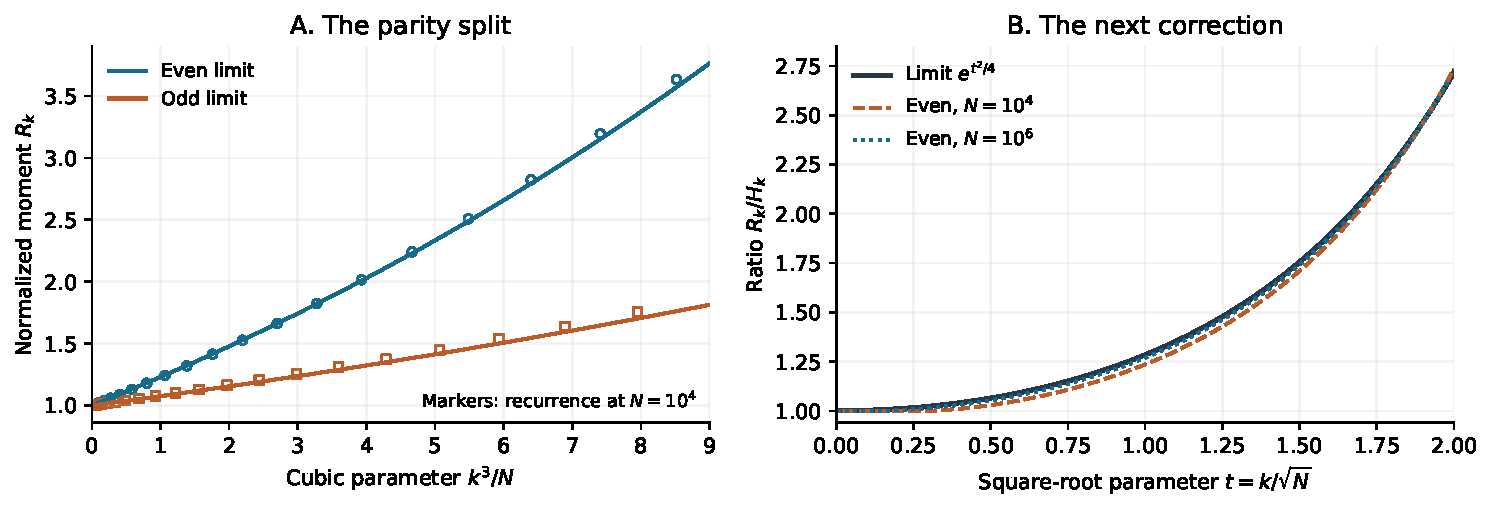
\includegraphics[width=\textwidth]{../figures/moment-regimes.pdf}
\caption{The two transitions. Left: the parity-dependent critical limits and recurrence evaluations at $N=10^4$. Right: the ratio to the hyperbolic approximation at even orders, compared with its square-root correction. Curves illustrate the proved statements and are not premises of the proofs.}
\label{fig:regimes}
\end{figure}

\section{The sublinear range and a formula at every order}\label{sec:asymptotics}

The square-root correction is the first term of a convergent exponent. Retaining that exponent describes every sublinear order. Keeping the permutation denominator exact then gives one formula throughout the full range $2\le k\le N$.

Define, for $0\le t<1$,
\begin{equation}\label{eq:actionG}
G(t)=t+\frac{t^2}{2}+(1-t^2)\log(1-t)-\frac23t^3
=\sum_{j\ge4}\frac{2t^j}{j(j-2)}.
\end{equation}
All coefficients in the last series are positive.

\begin{theorem}[Uniform sublinear approximation]\label{thm:sublinear}
For every sequence $b_N=o(N)$ with $b_N\ge2$,
\begin{equation}\label{eq:sublinear}
\sup_{2\le k\le b_N}
\left|\frac{R_k}{H_k\exp\{NG(\sqrt{k/N})\}}-1\right|
\longrightarrow0.
\end{equation}
The supremum is over integers. The definition of $H_k$ remains \eqref{eq:hyperdef}, including $K=k-1$ at odd orders.
\end{theorem}

\begin{corollary}[Sharp thresholds for successive corrections]\label{cor:hierarchy}
For a fixed integer $p\ge4$, put
\[
G_p(t)=\sum_{j=4}^{p}\frac{2t^j}{j(j-2)}.
\]
Along any sequence $2\le k=o(N)$,
\begin{equation}\label{eq:hierarchy}
\frac{R_k}{H_ke^{NG_p(\sqrt{k/N})}}\longrightarrow1
\quad\Longleftrightarrow\quad
k=o\left(N^{(p-1)/(p+1)}\right).
\end{equation}
The ratio stays bounded exactly when $k^{p+1}/N^{p-1}$ stays bounded. At $k/N^{(p-1)/(p+1)}\to c\in(0,\infty)$ its limit is
\begin{equation}\label{eq:hierarchyboundary}
\exp\left(\frac{2c^{(p+1)/2}}{(p+1)(p-1)}\right).
\end{equation}
In particular, the correction $e^{k^2/(4N)}$ is relatively accurate up to $k=o(N^{3/5})$. Adding $2k^{5/2}/(15N^{3/2})$ to its exponent extends that range to $k=o(N^{2/3})$.
\end{corollary}

The thresholds in \eqref{eq:hierarchy} are uniform upper-range statements as well: the relative error tends uniformly to zero on $2\le k\le b_N$ whenever $b_N=o(N^{(p-1)/(p+1)})$. The conclusion concerns each fixed truncation degree $p$.

\subsection{A coefficient estimate with both angular peaks controlled}

Write
\[
f(z)=\frac{z}{1-z}+\log(1-z),\qquad
x=\sqrt{K/N},\qquad r=\frac{x}{1+x}.
\]
The positive saddle and its variance parameter are explicit:
\begin{equation}\label{eq:saddleequation}
Nrf'(r)=\frac{Nr^2}{(1-r)^2}=K,\qquad
b=N(r\partial_r)^2f(r)=2K(1+x).
\end{equation}

\begin{lemma}[Uniform positive-saddle estimate]\label{lem:saddle}
Let $2\le K\le N$ be integers, $\epsilon\in\{0,1\}$ and $K+\epsilon\le N$. Put $\lambda=(2/3)Nx^3$. There is an absolute constant $C$ such that
\begin{equation}\label{eq:saddlecoefficient}
[z^{K+\epsilon}]e^{Nf(z)}
=\frac{e^{Nf(r)}r^{-K-\epsilon}}{\sqrt{2\pi b}}(1+E),
\qquad |E|\le C\left(K^{-1}+e^{-\lambda/8}\right).
\end{equation}
The right side is a relative approximation when $K$ and $\lambda$ diverge. The bound remains valid without that divergence.
\end{lemma}
\begin{proof}
Cauchy's formula reduces the normalized coefficient to
\[
\frac1{2\pi}\int_{-\pi}^{\pi}
e^{\Phi(\theta)-i\epsilon\theta}\,d\theta,
\qquad
\Phi(\theta)=N(f(re^{i\theta})-f(r))-iK\theta.
\]
The positive coefficients of $f$ give
\begin{equation}\label{eq:angulardamping}
-\Re\Phi(\theta)
\ge Nr^2\sin^2\theta+\frac23Nr^3(1-\cos3\theta).
\end{equation}
Here $r\le1/2$ and $Nr^2=K/(1+x)^2\ge K/4$. On $|\theta|\le\pi/6$,
\[
\Re\Phi(\theta)\le-\frac9{4\pi^2}K\theta^2.
\]
For each fixed $q\ge2$, the derivative sum
\[
N\sum_{j\ge2}\frac{j-1}{j}j^qr^j
\le K\sum_{j\ge2}\frac{j-1}{j}j^q2^{2-j}
\]
is bounded by an absolute constant depending only on $q$, times $K$. Taylor's inequalities and \eqref{eq:saddleequation} therefore give
\[
\Re\Phi=-b\theta^2/2+O(K\theta^4),\qquad
|\Im\Phi|\le CK|\theta|^3.
\]
Pair conjugate angles. The central integrand becomes
$e^{\Re\Phi}\cos(\Im\Phi-\epsilon\theta)$. Using
$|\cos u-1|\le u^2/2$ and the real exponential mean-value bound, its difference from $e^{-b\theta^2/2}$ is at most
\[
C(K\theta^4+K^2\theta^6+\theta^2)e^{-cK\theta^2}.
\]
Its integral is $O(K^{-3/2})$, whereas the Gaussian integral is of order $K^{-1/2}$. The Gaussian tails outside the central interval are exponentially small.

The pair term alone does not suppress the other peak. Write $\theta=\pi+u$ modulo $2\pi$, with $|u|\le\pi/6$. Then
\[
1-\cos3\theta=1+\cos3u\ge1,\qquad
\frac23Nr^3=\frac\lambda{(1+x)^3}\ge\frac\lambda8.
\]
The pair term in \eqref{eq:angulardamping} supplies Gaussian decay in $u$. The second-peak integral is therefore at most $CK^{-1/2}e^{-\lambda/8}$. At the remaining angles, $|\sin\theta|\ge1/2$ and the integral is at most $Ce^{-K/16}$. Dividing by the central Gaussian integral proves \eqref{eq:saddlecoefficient}. The circle $r\le1/2$ stays away from the singularity at one, including at $K=N$.
\end{proof}

\subsection{Restoring parity and the permutation denominator}

For the moment normalization take $K=2\lfloor k/2\rfloor=2m$ and $\epsilon=k-K$. Set
\begin{equation}\label{eq:actionq}
h(x)=x+(x^2-1)\log(1+x)-\frac{x^2}{2},\qquad
q(x)=h(x)-\frac23x^3.
\end{equation}
The action identity is exact:
\[
Nf(r)-K\log r+K\log x-K/2=Nh(x).
\]
Stirling's formula applied to $m!$ in $\mathcal L_k$, followed by Lemma~\ref{lem:saddle}, gives
\begin{equation}\label{eq:normalizedsaddle}
\frac{Q_k}{\mathcal L_k}
=\frac{e^{Nh(x)}(1+x)^{\epsilon-1/2}}{2\lambda^\epsilon}
\left[1+O\left(K^{-1}+e^{-\lambda/8}\right)\right].
\end{equation}
Indeed, the even factorial cancellation leaves $2^mm!N^{-m}$ times the coefficient. At odd orders the additional factor is exactly
\[
\frac3{2Kr}=\frac{1+x}{\lambda}.
\]
Thus no odd-order shift is lost. The exact hyperbolic term is
$H_k=(e^\lambda+(-1)^\epsilon e^{-\lambda})/(2\lambda^\epsilon)$.
When $K$ and $\lambda$ exceed sufficiently large fixed constants, taking logarithms in \eqref{eq:normalizedsaddle} yields
\begin{equation}\label{eq:logsaddle}
\log\frac{R_k}{H_k}
=\log D_k+Nq(x)+(\epsilon-1/2)\log(1+x)
+O\left(K^{-1}+e^{-\lambda/8}\right).
\end{equation}

For the sublinear formula, put $t=\sqrt{k/N}$ and
$I(u)=u+(1-u)\log(1-u)$. Monotonicity of $-\log(1-v)$ bounds its left Riemann sum by
\begin{equation}\label{eq:denominatorintegral}
0\le NI(k/N)-\log D_k\le-\log(1-k/N).
\end{equation}
The derivative identities
$h'(x)=2x\log(1+x)$ and $q'(x)=2x(\log(1+x)-x)$ give $|q'(x)|\le x^3$. Since $t^2-x^2=\epsilon/N$,
$N|q(t)-q(x)|\le k/N$. Finally, $I(t^2)+q(t)=G(t)$ exactly. Hence, uniformly for $k/N\le1/16$ under the same large-$K$, large-$\lambda$ conditions,
\begin{equation}\label{eq:logsublinear}
\log\frac{R_k}{H_k}
=NG(\sqrt{k/N})+(\epsilon-1/2)\log(1+\sqrt{K/N})
+O\left(k/N+K^{-1}+e^{-\lambda/8}\right).
\end{equation}
The parity term has order $\sqrt{k/N}$ and must be retained for finer error estimates.

\begin{proof}[Proof of Theorem~\ref{thm:sublinear}]
On $\sqrt N<k\le b_N=o(N)$, the minimum $K$ is of order $\sqrt N$ and the minimum $\lambda$ is of order $N^{1/4}$. Every error in \eqref{eq:logsublinear}, and its explicit parity term, tends uniformly to zero. On $2\le k\le\sqrt N$, Theorem~\ref{thm:sqrt} applies, while the positive series \eqref{eq:actionG} gives
\[
0\le NG(\sqrt{k/N})-\frac{k^2}{4N}
\le C\frac{k^{5/2}}{N^{3/2}}\le CN^{-1/4}.
\]
This patches the two ranges and includes fixed orders. It does not assume a single-saddle relative approximation when $\lambda$ is small.
\end{proof}

\begin{proof}[Proof of Corollary~\ref{cor:hierarchy}]
For fixed $p$, positivity and decreasing coefficients give
\[
G(t)-G_p(t)=\frac{2t^{p+1}}{(p+1)(p-1)}(1+O_p(t))
\quad(t\to0).
\]
The first term bounds the tail from below, and the same term divided by $1-t$ bounds it from above. Theorem~\ref{thm:sublinear} therefore gives
\[
\log\frac{R_k}{H_ke^{NG_p(\sqrt{k/N})}}
=\frac{2k^{(p+1)/2}}{(p+1)(p-1)N^{(p-1)/2}}
\bigl(1+O_p(\sqrt{k/N})\bigr)+o(1).
\]
This proves relative accuracy, its necessity, boundedness and the boundary limit. The same positive-tail bound proves uniformity over the stated upper ranges. In particular,
\[
NG(\sqrt{k/N})
=\frac{k^2}{4N}+\frac{2k^{5/2}}{15N^{3/2}}
+\frac{k^3}{12N^2}+\frac{2k^{7/2}}{35N^{5/2}}+\cdots.
\]
The coefficient $2/15$ combines block weights, pair depletion and the permutation denominator. It is not the raw weight of a single five-element block.
\end{proof}

\subsection{Keeping the denominator exact}

For $2\le k\le N$, define
\begin{equation}\label{eq:globalformula}
\mathcal A_{N,k}
=D_kH_k e^{Nq(\sqrt{K/N})}
(1+\sqrt{K/N})^{\epsilon-1/2}.
\end{equation}
Every factor is positive and finite, including at $k=N$.

\begin{theorem}[Uniform approximation at every order]\label{thm:global}
As $N\to\infty$,
\begin{equation}\label{eq:globalerror}
\sup_{2\le k\le N}\left|\frac{R_k}{\mathcal A_{N,k}}-1\right|
=O(N^{-1/4}).
\end{equation}
Uniformly for $\sqrt N\le k\le N$, the error is
$O(K^{-1}+e^{-\lambda/8})$, and hence $O(N^{-1/2})$.
\end{theorem}
\begin{proof}
Above $\sqrt N$, divide \eqref{eq:normalizedsaddle} by the exact $H_k$. The residual factor is $(1+(-1)^\epsilon e^{-2\lambda})^{-1}$. It differs from one exponentially little. The factor $D_k$ cancels exactly, so no approximation to $(N)_k$ is needed even at $k=N$.

Below $\sqrt N$, compare \eqref{eq:globalformula} to $e^{k^2/(4N)}H_k$. For $0\le x\le1/2$, integrating the elementary bounds on $\log(1+x)$ gives
\[
0\le q(x)+x^4/4\le2x^5/15.
\]
Also $0\le\log D_k-k(k-1)/(2N)\le k^3/(3N^2)$ for $k\le N/4$. The difference between $k(k-1)/(2N)$ and $(k^2+K^2)/(4N)$ is $-k/(2N)$ for even $k$ and $-1/(4N)$ for odd $k$. Thus, for $N\ge16$ and $2\le k\le\sqrt N$,
\[
\left|\log\frac{\mathcal A_{N,k}}{e^{k^2/(4N)}H_k}\right|
\le\frac{19}{30}N^{-1/4}+\frac56N^{-1/2}.
\]
Combine this with the explicit $O(N^{-1/4})$ estimate in Theorem~\ref{thm:rate}. This proves \eqref{eq:globalerror}. The global rate is not asserted to be optimal.
\end{proof}

At the top order, Lemma~\ref{lem:saddle} can be used with degree $K=N$ and offset zero, without a parity restriction on that lemma. Here $r=1/2$ and $b=4N$, giving
\[
[z^N]e^{Nf(z)}=\frac{e^N}{\sqrt{8\pi N}}(1+O(N^{-1})),\qquad
a_N(N)=\frac{1+O(N^{-1})}{2N!}.
\]
This endpoint also follows from the classical truncated-exponential identity for $L_N^{(-N-1)}$. It is a consistency check on the full-range formula, rather than a separate priority claim.

\section{The uniform rate and its sharp constant}\label{sec:rates}

The square-root correction has a uniform error of order $N^{-1/4}$. Its first signed term depends on parity, and the largest error has an explicit asymptotic constant. Retain $K=2\lfloor k/2\rfloor$, $\epsilon=k-K$ and $H_k$ from \eqref{eq:hyperdef}, and put
\begin{equation}\label{eq:rateW}
W_{N,k}=\frac{R_k}{e^{k^2/(4N)}H_k}.
\end{equation}

\begin{theorem}[An explicit uniform rate]\label{thm:rate}
For every fixed $C>0$,
\begin{equation}\label{eq:uniformrate}
\sup_{2\le k\le C\sqrt N}|W_{N,k}-1|=O_C(N^{-1/4}).
\end{equation}
More precisely, the explicit constants $A_i(C)$ in \eqref{eq:rateconstantsA} satisfy
\begin{equation}\label{eq:ratefinite}
|W_{N,k}-1|
\le A_1(C)N^{-1/4}+A_2(C)N^{-1/2}+A_3(C)N^{-1}
\end{equation}
whenever $N\ge16C^2$ and $2\le k\le C\sqrt N$. In addition, $A_1(C)\to0$ as $C\downarrow0$.
\end{theorem}

Appendix~\ref{sec:rateproof} proves the finite estimate, including fixed orders and the odd small-$\lambda$ regime. The constants are conservative. Their behavior as $C\downarrow0$ lets the following first correction remain uniform down to the smallest orders.

Define, for $c\ge0$,
\begin{equation}\label{eq:ratepsi}
\psi_\epsilon(c)=\frac{2\epsilon-1}{2}\sqrt c+\frac{2}{15}c^{5/2}.
\end{equation}

\begin{theorem}[Uniform first correction and sharp error constant]\label{thm:firstcorrection}
For every fixed $C>0$,
\begin{equation}\label{eq:uniformfirstcorrection}
\sup_{2\le k\le C\sqrt N}
\left|N^{1/4}(W_{N,k}-1)-\psi_{k\bmod2}(k/\sqrt N)\right|
\longrightarrow0.
\end{equation}
Consequently,
\begin{equation}\label{eq:sharprateconstant}
\lim_{N\to\infty}N^{1/4}
\sup_{2\le k\le C\sqrt N}|W_{N,k}-1|
=\frac{\sqrt C}{2}+\frac{2}{15}C^{5/2}.
\end{equation}
All suprema are over integers. Thus the order in \eqref{eq:uniformrate} is optimal for every fixed $C>0$.
\end{theorem}
\begin{proof}
Fix $0<d<C$. On $d\sqrt N\le k\le C\sqrt N$, the hypotheses of \eqref{eq:logsublinear} hold uniformly for sufficiently large $N$. Its remainder is $O_{C,d}(N^{-1/2})$. The series \eqref{eq:actionG} and the logarithm expansion give
\begin{align*}
NG(\sqrt{k/N})-\frac{k^2}{4N}
&=\frac{2k^{5/2}}{15N^{3/2}}+O_C(N^{-1/2}),\\
(\epsilon-1/2)\log(1+\sqrt{K/N})
&=\frac{2\epsilon-1}{2}\sqrt{k/N}+O_{C,d}(N^{-1/2}).
\end{align*}
The change from $K$ to $k$ in the second line costs at most a constant times $1/\sqrt{NK}$, which is smaller than the displayed remainder. Therefore
\[
\log W_{N,k}
=N^{-1/4}\psi_\epsilon(k/\sqrt N)+O_{C,d}(N^{-1/2}).
\]
The leading function is bounded on $[d,C]$. Exponentiation gives \eqref{eq:uniformfirstcorrection} uniformly on this restricted range.

For the remaining orders, \eqref{eq:ratefinite} with endpoint $d$ yields
\[
\limsup_{N\to\infty}N^{1/4}
\sup_{2\le k\le d\sqrt N}|W_{N,k}-1|\le A_1(d).
\]
Also $|\psi_\epsilon(c)|\le\sqrt d/2+2d^{5/2}/15$ for $0\le c\le d$. Split the full supremum at $d\sqrt N$, then let $d\downarrow0$. Since $A_1(d)\to0$, this proves \eqref{eq:uniformfirstcorrection}, including fixed orders and changing parity.

Finally,
\[
|\psi_0(c)|\le\psi_1(c)\le\psi_1(C)
=\frac{\sqrt C}{2}+\frac{2}{15}C^{5/2}
\qquad(0\le c\le C).
\]
The odd function is continuous and strictly increasing. Taking the largest odd integer $k_N\le C\sqrt N$ gives $k_N/\sqrt N\to C$. Equation~\eqref{eq:uniformfirstcorrection} supplies the matching lower limit, while its uniform bound supplies the upper limit. This proves \eqref{eq:sharprateconstant}.
\end{proof}

For example, at $k/\sqrt N\to1$, the signed limits are $-11/30$ along even orders and $19/30$ along odd orders. The sign change comes from the parity factor in \eqref{eq:logsublinear}. The positive $2c^{5/2}/15$ term is the first omitted term of the correction exponent. The sharp asymptotic constant in \eqref{eq:sharprateconstant} does not assert optimality of the finite constants $A_i(C)$.

\begin{figure}[htbp]
\centering
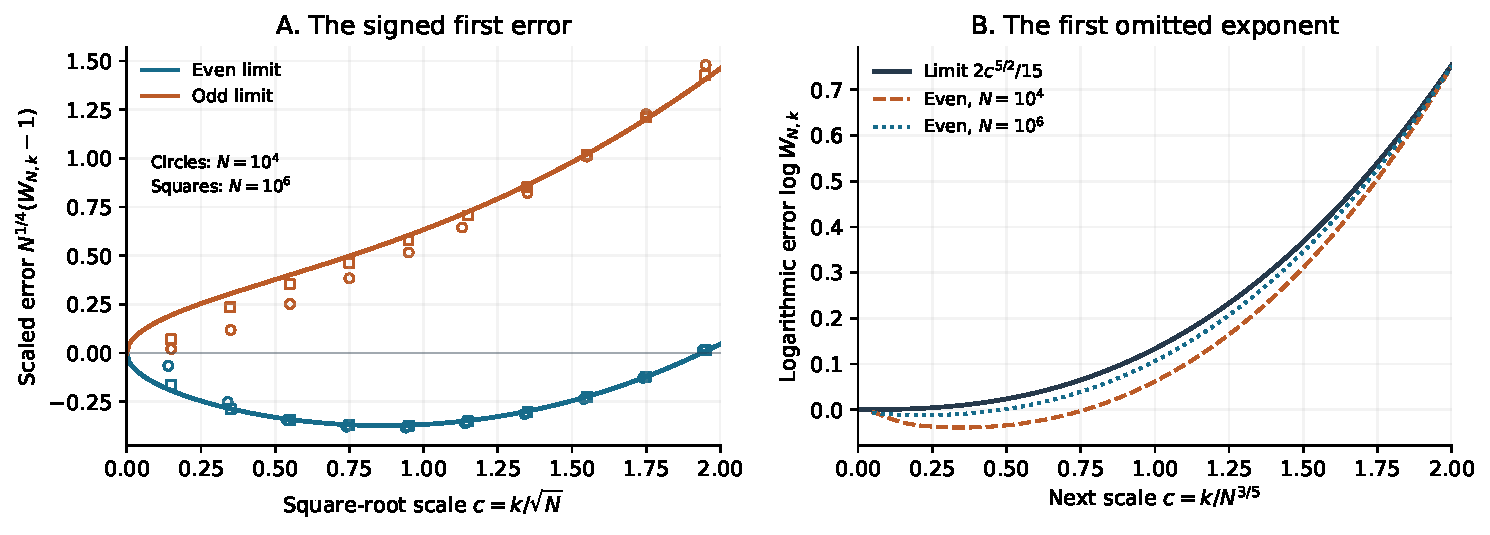
\includegraphics[width=\textwidth]{../figures/rate-and-hierarchy.pdf}
\caption{Two views of the next error. Left: the signed functions $\psi_0(c)$ and $\psi_1(c)$, compared with the positive recurrence at $N=10^4$ and $10^6$. Right: $\log W_{N,k}$ at $k\sim cN^{3/5}$ approaches $2c^{5/2}/15$. These finite evaluations corroborate the general theorems and are not used in their proofs.}
\label{fig:ratehierarchy}
\end{figure}

\section{Where the estimate enters spectral-gap arguments}\label{sec:spectral}

This section identifies the application of Theorem~\ref{thm:mixed} and explains the surrounding mechanism. The graph-level path enumeration and tangle estimates are separate ingredients from the papers cited below.

\subsection{Random lifts: one permutation per base edge}

In Bordenave's model, choose one orientation of each undirected edge of a finite base graph. Attach an independent uniform permutation of $[n]$ to each chosen edge. Its reverse orientation carries the inverse permutation. A lift edge between fibers is represented by a matrix entry of this permutation, and reversing the edge transposes the same entry.

Orient every factor in a requested product according to the chosen base orientations. Base edges become colors in \eqref{eq:product}. Distinct requested lift edges become distinct cells. Their multiplicities and consistency conditions are unchanged. The parameter $a_1$ of \cite[Proposition 28]{Bordenave} is exactly $h$ here, and its inconsistent centered-singleton count is $b$.

If the original product has $k$ factors, then $a\le k\le\sqrt n$. For $a\ge2$, Corollary~\ref{cor:mixedscalar} gives
\[
|\E P|\le\sqrt e\,2^bn^{-a}(2\sqrt{a/n})^{a_1}
\le\sqrt e\,2^bn^{-a}(3k/\sqrt n)^{a_1}.
\]
The case $a=1$ is covered directly by the theorem. This proves the stated product estimate in Proposition 28, with a stronger consistent-singleton factor.

\subsection{Biregular graphs: the size is the half-edge count}

Take a bipartite configuration model with $n_L$ left vertices of degree $d_L$ and $n_R$ right vertices of degree $d_R$. The two half-edge sets both have size
\[
L=n_Ld_L=n_Rd_R.
\]
A uniform matching between them is a uniform permutation of $[L]$. Its symmetric half-edge matching matrix has the block form
\[
\begin{pmatrix}0&U\\U^{\mathsf T}&0\end{pmatrix},
\]
where $U$ is a uniform $L$ by $L$ permutation matrix. Same-side entries of the matching matrix and its centered version vanish, so any product containing them is zero. Orient each remaining requested matching factor from left to right. Theorem~\ref{thm:mixed} applies with $n=L$, exactly as needed in \cite[preprint Lemma 7, published Lemma 5.6]{BDH}. The centering is $1/L$, not $1/n_L$ or $1/n_R$.

This model differs from an unrestricted perfect matching of a single set of half-edges. That latter model is treated by Bordenave's Proposition 11. The off-diagonal bipartite block is what makes Proposition 28 the correct input here.

\subsection{Why isolated centered factors help a trace expansion}

The non-backtracking matrix is indexed by oriented graph edges. Its entry from an oriented edge $e$ to an oriented edge $f$ is one exactly when the head of $e$ is the tail of $f$ and $f$ is not the reverse of $e$. This definition permits a return along a different parallel edge. In a simple graph, it reduces to $v=x$ and $y\ne u$ for consecutive edges $u\to v$ and $x\to y$. Thus powers of the matrix count walks that never immediately reverse the same edge.

The matrix is generally not normal. A safe norm estimate uses
\[
\|C\|^{2s}\le\tr\bigl((CC^*)^s\bigr).
\]
Expanding the right side for a centered path matrix produces products of matching entries. A product that uses $a$ distinct matches starts at scale $L^{-a}$. Each consistent centered singleton gives an additional factor of order $\sqrt{a/L}$ in our bound. Repeated cells and conflicting singletons have different costs and must be counted separately.

Choosing locations for a circuit contributes positive powers of the graph size. Matching probabilities cancel most of them. Excess cycles and isolated centered factors supply the savings that remain. The combinatorial argument must sum these estimates over all allowed circuit shapes. The mixed-product theorem handles each fixed pattern, but does not perform this sum.

Short neighborhoods are typically tree-like, with a controlled allowance for a single cycle. The papers restrict to such paths and estimate the remainder from more complicated local tangles. Non-backtracking walks make this separation useful because immediate reversals would create many large, uninformative contributions even on a tree.

\subsection{The algebraic bridge back to adjacency}

For a finite simple graph with adjacency matrix $A$, degree matrix $D$ and non-backtracking matrix $B$, the determinant identity of Ihara and Bass in the cited papers reads
\begin{equation}\label{eq:ihara}
\det(I-uB)=(1-u^2)^{|E|-|V|}\det\bigl(I-uA+u^2(D-I)\bigr).
\end{equation}
For a $d$-regular graph with $d\ge2$, this reduces, away from the exceptional roots, to
\[
\lambda=z+\frac{d-1}{z}.
\]
The circle $|z|=\sqrt{d-1}$ corresponds to the adjacency interval $[-2\sqrt{d-1},2\sqrt{d-1}]$. An adjacency eigenvalue outside that interval produces a non-backtracking root outside the circle.

For a bipartite biregular graph write
\[
A=\begin{pmatrix}0&X\\X^{\mathsf T}&0\end{pmatrix},\qquad
\alpha=d_L-1,\quad\gamma=d_R-1,
\]
and assume $d_L,d_R\ge2$. If $s>0$ is a singular value of $X$, the relevant block of \eqref{eq:ihara} yields
\begin{equation}\label{eq:biregularbridge}
(z^2+\alpha)(z^2+\gamma)=s^2z^2.
\end{equation}
Putting $x=z^2$ gives the scalar map
\begin{equation}\label{eq:scalarbridge}
s^2=x+\frac{\alpha\gamma}{x}+\alpha+\gamma.
\end{equation}
The circle $|x|=\sqrt{\alpha\gamma}$ corresponds to
\[
|\sqrt\alpha-\sqrt\gamma|\le s\le\sqrt\alpha+\sqrt\gamma.
\]
If $s>\sqrt\alpha+\sqrt\gamma$, the quadratic in $x$ has a positive root greater than $\sqrt{\alpha\gamma}$, so $|z|>(\alpha\gamma)^{1/4}$. This is the precise route by which a non-backtracking bound excludes adjacency outliers. Rectangular nullspaces can also produce zero adjacency eigenvalues, which are outside this positive-singular-value calculation.

For example, degrees $(3,7)$ give the positive bulk interval $[\sqrt6-\sqrt2,\sqrt6+\sqrt2]$, approximately $[1.035,3.864]$, while the trivial singular value is $\sqrt{21}\approx4.583$. The spectral theorem controls the remaining singular values asymptotically with high probability. Our proof supplies its matching-product input, not a replacement for all its graph-level estimates.

\section{Two checks on a conditioning formula}\label{sec:conditioning}

The following examples concern equation (62) on printed page 1428 of Bordenave's published article \cite{Bordenave}. The same formula appears on page 38 of arXiv version 4. They refute that intermediate conditional assertion under its displayed conditioning. They are not counterexamples to Proposition 28, which appears on printed page 1426 and which Section~\ref{sec:mixed} proves by a different argument.

For requested cells $y_t=(i_t,j_t)$, the source conditions on
\[
\mathcal F_t=\sigma\bigl(\sigma(i_s),\sigma^{-1}(j_s):s\ne t\bigr)
\]
and asserts a probability of the form
\[
\PP(M_{i_tj_t}=1\mid\mathcal F_t)
=\frac{\1_{\Omega_t^c}}{n_t}\le\frac1{n-a+1},
\qquad
n_t=n-|\{\sigma(i_s):s\ne t\}|.
\]
The event $\Omega_t$ holds if some $s\ne t$ satisfies $\sigma(i_s)=j_t$ or $\sigma^{-1}(j_s)=i_t$.

\begin{example}[A shared row reveals the cell]
Let $n=4$, $y_1=(1,1)$ and $y_2=(1,2)$. Then $a=k=2\le\sqrt n$, and $\mathcal F_1$ includes $\sigma(1)$. On the event $\sigma(1)=1$, of probability $1/4$, the actual conditional probability of $M_{11}=1$ is one. The displayed event $\Omega_1$ also holds, because $\sigma(i_2)=j_1$. The source formula therefore gives zero. Its claimed upper bound $1/3$ fails as well.
\end{example}

\begin{example}[Images and preimages remove two arrows]
Let $n=4$, $y_1=(1,1)$ and $y_2=(2,2)$. Condition on
\[
\sigma(2)=3,\qquad \sigma^{-1}(2)=4.
\]
This event has probability $1/12$. It exposes two arrows, $2\mapsto3$ and $4\mapsto2$. The remaining rows are $1,3$ and the remaining columns are $1,4$. Thus
\[
\PP(M_{11}=1\mid\mathcal F_1)=\frac12.
\]
Neither clause of $\Omega_1$ holds, but the displayed $n_t$ is $4-1=3$. The source formula gives $1/3$, and the proposed bound $1/(n-a+1)$ also gives $1/3$.
\end{example}

The second example shows that merely requiring the tested cell to be unrevealed does not repair the formula. One must count every removed row and column under the actual conditioning. Section~\ref{sec:mixed} avoids the issue by exposing only a compatible prescribed set. Its remaining dimension is exactly $n-r$.

\section{Contribution, limitations and further questions}

The mixed-product theorem identifies an attained maximum when there is no inconsistent centered singleton. Its proof keeps the exact depleted moment, merges colors through positive partition weights, and handles arbitrary multiplicities through affine indicator identities. The scalar consequences recover the spectral estimate with a smaller singleton factor and an optimal universal prefactor. The diagonal results determine the original cubic threshold, the parity transition, a hierarchy of further corrections and the sharp first uniform error.

The base recurrence, its normalized parity form and the leading coefficients belong to Collins and Nagatsu \cite{CN}. The mixed estimate itself is already part of Bordenave's spectral-gap method \cite{Bordenave}. The special-function identities and the saddle method are classical. The precise refinements proved here are the attained envelope at fixed support and singleton counts, the necessity and bounded-comparability characterization of the cubic scale, the uniform sublinear correction hierarchy, and the sharp parity-dependent error on bounded square-root ranges. A targeted literature check found no exact duplicate of these statements, but cannot certify the absence of every earlier equivalent formula.

Bordenave and Zhu \cite[Lemma 2.1]{BZ} retain the original singleton factor $3k/\sqrt N$ and explicitly bound the raw factorial ratio by $\sqrt e$ in their equation (2.3). That elementary bound is a known ingredient here. Our exact refinement retains $\mu_h(n,a-h)$ in addition to $F_n(a-h)$. The factor $\Gamma_{n,a,h}$ is a scalar upper bound on that moment and is smaller than $\beta$ when $h<a$. The attained-maximum assertion concerns $b=0$. We do not claim that $2^b$ is sharp for prescribed $b>0$.

The Laguerre representation makes the parameter regime precise: the degree is $k$, the parameter is $\alpha=-N-1$, and the argument is $-N$. Thus $-\alpha/k\to\infty$ throughout the sublinear range. Kuijlaars and McLaughlin \cite{KM}, and the regime described by Dai and Wong \cite{DW}, treat a finite limiting ratio greater than one. Those results overlap the macroscopic part of our full-range formula, so that part is not presented as a new special-function asymptotic regime. Theorem 1 of Dai, Ismail and Wang \cite{DIW} assumes $\alpha>0$ when $\alpha/k\to\infty$. In the inspected preprint of Dunster, Gil and Segura \cite[Section 1, equation (1.6) and Cases 1a, 1b and 2]{DGS}, $\alpha=(k+1/2)(a^2-1)$ with $a\ge0$, excluding $\alpha=-N-1$ for $k\le N$. These parameter comparisons do not turn analytic continuation into a uniform error estimate.

At $k=N$, the identity with a truncated exponential is classical, as recorded in \cite[Section 1]{DMO}. The contribution of Theorem~\ref{thm:global} is a self-contained formula that patches fixed orders, the parity transition and the endpoint while keeping $(N)_k$ exact. Its stated $O(N^{-1/4})$ global bound is not asserted to be optimal. The sharp rate in Section~\ref{sec:rates} concerns the different, quartically corrected hyperbolic approximation.

The inequalities are proved symbolically for their stated parameter ranges. Exact finite computations check normalization, the depleted recurrence and the conditioning examples. Numerical plots illustrate the asymptotic regimes. Neither kind of computation is used as a substitute for a general proof.

The remaining graph-level task is to combine the sharper cell-pattern estimate with circuit enumeration and tangle remainders while retaining the degree dependence. A better estimate for one fixed product does not automatically improve a spectral theorem: the patterns that dominate the full sum must be identified first. The present paper does not assert a new second-eigenvalue bound or an end-to-end audit of either random-graph proof.

\appendix
\section{Explicit constants and proof of the uniform rate}\label{sec:rateproof}

We prove Theorem~\ref{thm:rate} without a lower bound on the moment order or the hyperbolic parameter. Throughout this appendix,
\[
m=\lfloor k/2\rfloor,\quad K=2m,\quad\epsilon=k-K,\quad
\lambda=\frac23\sqrt{K^3/N},\quad
\delta=\frac{K^2}{N},\quad\eta=\frac{3K^2}{4N}.
\]
The symbol $\delta$ here denotes the scale parameter, not parity.

\subsection{Constants and a finite estimate}

For $C>0$, put $a=3C^2/4$ and define
\begin{equation}\label{eq:rateconstantsB}
\begin{aligned}
B_1(C)&=\frac43(2+3a)\sqrt C+\frac{2144}{27}C^{5/2},\\
B_2(C)&=\frac32(2a+3)C
+\frac{16}{9}(245+45a+45a^2)C,\\
B_3(C)&=3(10a^3+188a^2+457a+141).
\end{aligned}
\end{equation}
One valid choice in \eqref{eq:ratefinite} is
\begin{equation}\label{eq:rateconstantsA}
\begin{aligned}
A_1(C)&=e^{7C^2/4}B_1(C)+2e^{11C^2/4}C^{5/2},\\
A_2(C)&=e^{7C^2/4}B_2(C)+2e^{11C^2/4}C
+e^{C^2/3}\left(\frac C2+\frac{C^3}{3}\right),\\
A_3(C)&=e^{7C^2/4}B_3(C).
\end{aligned}
\end{equation}
In particular, the displayed expression for $A_1(C)$ tends to zero as $C\downarrow0$.

We first prove a bound using the actual order $k$. For $2\le k\le N/4$, set
\[
b=\min(\lambda,\lambda^2),\qquad
r=\frac{k}{2N}+\frac{k^3}{3N^2},\qquad
\tau=\frac{2K^{5/2}}{N^{3/2}},\qquad\zeta=\frac{2K}{N},
\]
and
\begin{equation}\label{eq:rateB}
\begin{aligned}
\mathcal B={}&\frac{(2+3\eta)b+2\eta^2+3\eta}{m}\\
&+\frac{1}{m^2}\bigl[67\lambda^3+(245+45\eta+45\eta^2)\lambda^2\\
&\hspace{27mm}+10\eta^4+188\eta^3+457\eta^2+141\eta\bigr].
\end{aligned}
\end{equation}
The finite estimate is
\begin{equation}\label{eq:ratelocal}
|W_{N,k}-1|
\le e^r-1+D_ke^{-k^2/(4N)+\eta}
\bigl[\mathcal B+(1+\zeta)e^\tau-1\bigr].
\end{equation}

\subsection{Condition the triple count on its parity}

Let $J$ be Poisson with mean $\lambda$, conditioned to have parity $\epsilon$. Independently let $V$ be Poisson with mean $\eta$. Put
\[
T=J-\epsilon,\qquad S=3T/2+2V,
\]
and define
\[
w_\epsilon(s)=\frac{(m-\epsilon)_s}{m^s}
\quad(0\le s\le m-\epsilon),
\]
with value zero at larger nonnegative integers. The variables $T$ and $S$ are nonnegative integers. Restricting \eqref{eq:availabilityeven} and \eqref{eq:availabilityodd} to blocks of sizes two, three and four shows that their contribution to $(Q_k/\mathcal L_k)/H_k$ is exactly
\begin{equation}\label{eq:rateconditioned}
e^\eta\E w_\epsilon(S).
\end{equation}
At odd orders, the $1/\lambda$ factors in the coefficient formula and $H_k$ cancel. Thus \eqref{eq:rateconditioned} is valid even when $\lambda$ is small.

The following bounds hold for both conditioned laws:
\begin{align}
\E T&\le b,&
|\E T^2-\lambda^2|&\le b,&
\E T^2&\le2\lambda^2,\label{eq:ratemomentsone}\\
\E T^3&\le\lambda^3+4\lambda^2,&
\E(T^2-\lambda^2)^2&\le4\lambda^3+8\lambda^2.
&&\label{eq:ratemomentstwo}
\end{align}
For verification, write $v=\lambda\tanh\lambda$ and $q=\lambda\coth\lambda-1$. Differentiating the normalizers $\cosh\lambda$ and $\sinh\lambda$ gives
\[
\begin{array}{c|cc}
&\epsilon=0&\epsilon=1\\ \hline
\E T&v&q\\
\E T^2&\lambda^2+v&\lambda^2-q\\
\E T^3&\lambda^2v+3\lambda^2+v&\lambda^2+\lambda^2q+q\\
\E(T^2-\lambda^2)^2&4\lambda^2v+7\lambda^2+v&3\lambda^2+(4\lambda^2-1)q
\end{array}
\]
Both $v$ and $q$ lie in $[0,b]$. For $q$, use $\coth\lambda\le1+1/\lambda$ and
$\lambda\cosh\lambda\le(1+\lambda^2)\sinh\lambda$. The latter inequality follows by differentiation, since the difference is zero at zero and has derivative $\lambda^2\cosh\lambda+\lambda\sinh\lambda\ge0$. The table now proves \eqref{eq:ratemomentsone} and \eqref{eq:ratemomentstwo}.

\subsection{Compare pair availability with an exponential}

For an integer $s\ge0$, set $A(s)=s(s-1+2\epsilon)/(2m)$. Then
\begin{equation}\label{eq:rateavailability}
0\le e^{-A(s)}-w_\epsilon(s)\le4s^3/m^2.
\end{equation}
If $s\le m/2$, expand the logarithm of the product. Its linear sum is $-A(s)$, and
\[
0\le-\log(1-u)-u\le\frac{u^2}{2(1-u)}
\]
bounds the remaining sum by $s^3/m^2$. Use $1-e^{-z}\le z$ to obtain \eqref{eq:rateavailability}. If $s>m/2$, the difference lies in $[0,1]$ and $4s^3/m^2>1$, including when the product is assigned zero.

Write $A=A(S)$. Since $\delta=9\lambda^2/(8m)$,
\begin{equation}\label{eq:rateAexpand}
A-\delta
=\frac{9(T^2-\lambda^2)}{8m}+\frac{3TV}{m}+\frac{2V^2}{m}
+(2\epsilon-1)\left(\frac{3T}{4m}+\frac Vm\right).
\end{equation}
Independence and the Poisson moments
\[
\E V^2=\eta^2+\eta,\quad
\E V^3=\eta^3+3\eta^2+\eta,\quad
\E V^4=\eta^4+6\eta^3+7\eta^2+\eta
\]
give
\begin{equation}\label{eq:rateAmean}
|\E A-\delta|
\le\frac{(15/8+3\eta)b+2\eta^2+3\eta}{m}.
\end{equation}
Apply $(u_1+\cdots+u_5)^2\le5\sum_i u_i^2$ to the five terms in \eqref{eq:rateAexpand}. Equations~\eqref{eq:ratemomentsone} and \eqref{eq:ratemomentstwo} then imply
\begin{equation}\label{eq:rateAsecond}
\begin{aligned}
\E(A-\delta)^2\le\frac5{m^2}\bigl[&\frac{81}{16}\lambda^3
+(45/4+18\eta+18\eta^2)\lambda^2\\
&+4\eta^4+24\eta^3+29\eta^2+5\eta\bigr].
\end{aligned}
\end{equation}
Also $(u+v)^3\le4(u^3+v^3)$ for nonnegative $u,v$ gives
\begin{equation}\label{eq:rateSthird}
\E S^3\le\frac{27}{2}(\lambda^3+4\lambda^2)
+32(\eta^3+3\eta^2+\eta).
\end{equation}

Because $A,\delta\ge0$ and the second derivative of $e^{-u}$ has absolute value at most one on this interval, Taylor's theorem yields
\[
|\E e^{-A}-e^{-\delta}|
\le|\E A-\delta|+\tfrac12\E(A-\delta)^2.
\]
Combine this with \eqref{eq:rateavailability} and \eqref{eq:rateAmean} through \eqref{eq:rateSthird}. Rounding the positive coefficients upward gives
\begin{equation}\label{eq:ratewerror}
|\E w_\epsilon(S)-e^{-\delta}|\le\mathcal B.
\end{equation}
For example, the coefficient of $\lambda^3/m^2$ before rounding is $54+405/32=2133/32<67$, and that of $\lambda^2/m^2$ independent of $\eta$ is $1953/8<245$.

\subsection{Larger blocks and the denominator}

Let $x=\sqrt{K/N}\le1/2$ and $\lambda_j=N(j-1)x^j/j$. Denote by $T_{\rm e}$ and $T_{\rm o}$ the sums of these weights over even and odd $j\ge5$. Then
\[
T_{\rm e}+T_{\rm o}\le\frac{Nx^5}{1-x}\le\tau,
\qquad
\frac{T_{\rm o}}\lambda\le\frac{3x^2}{2(1-x^2)}\le\zeta.
\]
All coefficients are nonnegative. Removing availability factors bounds the additional contribution after division by $H_k$ by
\[
e^\eta(e^\tau-1)
\quad\text{at even orders},\qquad
e^\eta\bigl[(1+\zeta)e^\tau-1\bigr]
\quad\text{at odd orders}.
\]
Indeed, summing the added odd weights replaces $\cosh\lambda$ or $\sinh\lambda$ by its value at $\lambda+T_{\rm o}$. The logarithmic derivative of $\cosh u$ is at most one, as is that of $\sinh u/u$. The latter gives the extra factor $1+T_{\rm o}/\lambda$ and preserves the small-$\lambda$ normalization.

Together with \eqref{eq:rateconditioned} and \eqref{eq:ratewerror}, this proves
\begin{equation}\label{eq:rateQerror}
\left|\frac{Q_k/\mathcal L_k}{H_k}-e^{\eta-\delta}\right|
\le e^\eta\bigl[\mathcal B+(1+\zeta)e^\tau-1\bigr].
\end{equation}
Since $\eta-\delta=-K^2/(4N)$, the central value after restoring $D_k$ and the correction in \eqref{eq:rateW} is
$D_k\exp(-(k^2+K^2)/(4N))$.
The logarithm remainder inequality gives, for $k\le N/4$,
\[
0\le\log D_k-\frac{k(k-1)}{2N}\le\frac{k^3}{3N^2}.
\]
The difference between $k(k-1)/(2N)$ and $(k^2+K^2)/(4N)$ is $-k/(2N)$ for even $k$ and $-1/(4N)$ for odd $k$. Thus its total logarithmic error has absolute value at most $r$. Multiplying \eqref{eq:rateQerror} by $D_ke^{-k^2/(4N)}$ proves \eqref{eq:ratelocal}.

\subsection{Uniform bounds for every positive endpoint}

Assume $C>0$, $N\ge16C^2$ and $2\le k\le C\sqrt N$. Then $k\le N/4$, $K\le C\sqrt N$, $\eta\le a$ and $\delta\le C^2$. The identities
\[
\frac\lambda m=\frac43\sqrt{K/N},\quad
\frac\eta m=\frac{3K}{2N},\quad
\frac{\lambda^3}{m^2}=\frac{32K^{5/2}}{27N^{3/2}},\quad
\frac{\lambda^2}{m^2}=\frac{16K}{9N},\quad
\frac\eta{m^2}=\frac3N
\]
show, using $b\le\lambda$, that
\[
\mathcal B\le B_1(C)N^{-1/4}+B_2(C)N^{-1/2}+B_3(C)N^{-1}.
\]
Moreover, $\tau\le\delta\le C^2$, so
\[
(1+\zeta)e^\tau-1
\le e^{C^2}(\tau+\zeta)
\le2e^{C^2}\bigl(C^{5/2}N^{-1/4}+CN^{-1/2}\bigr).
\]
The multiplier $D_ke^{-k^2/(4N)+\eta}$ in \eqref{eq:ratelocal} is at most $e^{7C^2/4}$ because $\log D_k\le k^2/N$. Finally,
\[
r\le\left(\frac C2+\frac{C^3}{3}\right)N^{-1/2},\qquad
r=\frac{k^2}{N}\left(\frac1{2k}+\frac{k}{3N}\right)\le\frac{C^2}{3}.
\]
Hence $e^r-1\le e^{C^2/3}(C/2+C^3/3)N^{-1/2}$. Substitution in \eqref{eq:ratelocal} gives precisely \eqref{eq:rateconstantsA} and proves \eqref{eq:ratefinite}. These comparisons use only $C>0$, not $C\ge1$. They also justify the small-endpoint limit of $A_1$ used in Theorem~\ref{thm:firstcorrection}.

\begin{thebibliography}{99}
\bibitem{Bordenave}
C. Bordenave, \emph{A new proof of Friedman's second eigenvalue theorem and its extension to random lifts}, Annales scientifiques de l'\'Ecole normale sup\'erieure (4) 53(6) (2020), 1393 to 1439.
\href{https://doi.org/10.24033/asens.2450}{doi:10.24033/asens.2450}.
\href{https://smf.emath.fr/download/pdf/1498332}{Published full text}. Proposition 28 is on page 1426 and equation (62) on page 1428. The same numbers occur in \href{https://arxiv.org/abs/1502.04482v4}{arXiv:1502.04482v4}.
\bibitem{BDH}
G. Brito, I. Dumitriu and K. D. Harris, \emph{Spectral gap in random bipartite biregular graphs and applications}, Combinatorics, Probability and Computing 31(2) (2022), 229 to 267.
\href{https://doi.org/10.1017/S0963548321000249}{doi:10.1017/S0963548321000249}.
\href{https://arxiv.org/abs/1804.07808v6}{arXiv:1804.07808v6}. Lemma 7 in this preprint is Lemma 5.6 in the published article.
\bibitem{CN}
B. Collins and M. Nagatsu, \emph{Weingarten calculus for centered random permutation matrices}, Algebraic Combinatorics 9(2) (2026), 465 to 479.
\href{https://doi.org/10.5802/alco.480}{doi:10.5802/alco.480}.
\bibitem{Friedman}
J. Friedman, \emph{A proof of Alon's second eigenvalue conjecture and related problems}, Memoirs of the American Mathematical Society 195 (2008), no. 910.
\href{https://arxiv.org/abs/cs/0405020}{arXiv:cs/0405020}.
\bibitem{BC}
C. Bordenave and B. Collins, \emph{Eigenvalues of random lifts and polynomials of random permutation matrices}, Annals of Mathematics 190(3) (2019), 811 to 875.
\href{https://doi.org/10.4007/annals.2019.190.3.3}{doi:10.4007/annals.2019.190.3.3}.
\bibitem{DLMF}
NIST Digital Library of Mathematical Functions, Laguerre polynomials,
\href{https://dlmf.nist.gov/18.5.E12}{equation 18.5.12} and
\href{https://dlmf.nist.gov/18.12.E13}{equation 18.12.13}. Accessed November 14, 2026.
\bibitem{DW}
D. Dai and R. Wong, \emph{Global asymptotics for Laguerre polynomials with large negative parameter: a Riemann-Hilbert approach}, The Ramanujan Journal 16(2) (2008), 181 to 209.
\href{https://doi.org/10.1007/s11139-007-9108-7}{doi:10.1007/s11139-007-9108-7}.
\bibitem{DIW}
D. Dai, M. E. H. Ismail and J. Wang, \emph{Asymptotics for Laguerre polynomials with large order and parameters}, Journal of Approximation Theory 193 (2015), 4 to 19.
\href{https://doi.org/10.1016/j.jat.2014.03.009}{doi:10.1016/j.jat.2014.03.009}.
\bibitem{BZ}
C. Bordenave and Y. Zhu, \emph{A second eigenvalue lower bound for the directed configuration model}, preprint, 2026.
\href{https://arxiv.org/abs/2611.07104v1}{arXiv:2611.07104v1}.
\bibitem{KM}
A. B. J. Kuijlaars and K. T.-R. McLaughlin, \emph{Riemann-Hilbert analysis for Laguerre polynomials with large negative parameter}, Computational Methods and Function Theory 1 (2001), 205 to 233.
\href{https://arxiv.org/abs/math/0204248v1}{arXiv:math/0204248v1}.
\bibitem{DGS}
T. M. Dunster, A. Gil and J. Segura, \emph{Uniform asymptotic expansions for Laguerre polynomials and related confluent hypergeometric functions}, Advances in Computational Mathematics 44(5) (2018), 1441 to 1474.
\href{https://doi.org/10.1007/s10444-018-9589-5}{doi:10.1007/s10444-018-9589-5}.
\href{https://arxiv.org/abs/1705.01190v1}{arXiv:1705.01190v1}.
\bibitem{DMO}
C. D\'iaz Mendoza and R. Orive, \emph{The Szeg\H{o} curve and Laguerre polynomials with large negative parameters}, Journal of Mathematical Analysis and Applications 379(1) (2011), 305 to 315.
\href{https://doi.org/10.1016/j.jmaa.2010.12.053}{doi:10.1016/j.jmaa.2010.12.053}.
\href{https://arxiv.org/abs/1011.2017v1}{arXiv:1011.2017v1}.
\end{thebibliography}
\end{document}
